% ==================== CHAPTER 3: REALIZATION AND EXPERIMENTATION ====================
\chapter{Realization and Experimentation}
\setcounter{section}{0}

\section*{Introduction}
\addcontentsline{toc}{section}{Introduction}

\initial{T}his chapter presents the practical realization of the IoT-REAP platform. It describes the development environment, the technologies and tools used, and the principal interfaces implemented for public users, learners, teachers, engineers, and administrators.

\section{Tools and Development Environment}

The implementation of IoT-REAP required a development environment capable of supporting backend web application development, reactive frontend interfaces, virtual machine orchestration, and industrial remote access workflows. The working environment therefore combined hardware resources suitable for local development and testing with a modern software stack centered on Laravel, React, TypeScript, and MySQL.

\subsection{Hardware Environment}

The hardware environment used for IoT-REAP development was organized around three complementary layers: the developer workstation, the application execution environment, and the remote infrastructure targeted by the platform. The development workstation had to be powerful enough to run a local PHP application server, a Node.js asset pipeline, a relational database, code editors, and testing tools simultaneously. In addition, the project domain required an infrastructure context involving virtual machines, gateway nodes, cameras, and remotely accessible lab equipment.

\begin{table}[H]
\centering
\caption{Hardware Environment for IoT-REAP Development and Execution}
\label{tab:hardware-env}
\begin{tabular}{|p{4cm}|p{10.5cm}|}
\hline
\textbf{Hardware Element} & \textbf{Role in the Project} \\
\hline
Developer Workstation & Used for source code editing, frontend compilation, backend execution, database interaction, and local testing of the Laravel and React application. \\
\hline
Application Server Environment & Hosts the Laravel application, queue workers, scheduled tasks, and the built frontend assets required by the platform. \\
\hline
Database Server & Stores users, training paths, training units, quizzes, payments, notifications, reservations, sessions, and other persistent business data. \\
\hline
Virtualization Infrastructure & Provides the virtual machines launched for hands-on practical sessions and browser-based remote access scenarios. \\
\hline
Remote Access Infrastructure & Includes services used to expose clientless access to provisioned lab machines and remote training environments through the browser. \\
\hline
Industrial and IoT Equipment & Represents the target equipment domain of the platform, including cameras, hardware gateways, USB devices, and operational training resources. \\
\hline
\end{tabular}
\end{table}

\subsection{Software Environment}

The software environment brought together development tools, dependency managers, testing utilities, and collaboration platforms. Since IoT-REAP is implemented as a Laravel application using Inertia.js and React, both PHP and JavaScript tooling were required throughout the development cycle.

\begin{table}[H]
\centering
\caption{Software Development Environment}
\label{tab:software-env}
\begin{tabular}{|p{3.7cm}|p{3cm}|p{7.8cm}|}
\hline
\textbf{Name} & \textbf{Category} & \textbf{Role in the Project} \\
\hline
Visual Studio Code & Code Editor & Used as the main development environment for editing PHP, TypeScript, React, route definitions, configuration files, and LaTeX report sources. \\
\hline
Laravel Herd & Local Server & Used as a lightweight local development environment for running the Laravel application, PHP runtime, and MySQL database during implementation. \\
\hline
Git and GitHub & Version Control & Used to manage source code history, feature evolution, collaboration, and recovery of stable project states during iterative development. \\
\hline
Composer & PHP Dependency Manager & Used to install and manage Laravel framework packages and backend dependencies such as Fortify, Inertia Laravel, Socialite, and Stripe integration libraries. \\
\hline
NPM & JavaScript Dependency Manager & Used to manage frontend dependencies including React, TypeScript, Vite, Tailwind CSS, Radix UI components, Zustand, React Query, and Vitest. \\
\hline
Vite & Build Tool & Used for frontend asset bundling, hot module replacement in development, and production asset compilation. \\
\hline
MySQL & Database System & Used for relational data persistence, including authentication data, training content, reservations, operational sessions, and administrative records. \\
\hline
DBeaver & Database Management & Used for visual database inspection, query execution, schema browsing, and data verification during development and debugging. \\
\hline
Docker & Containerization & Used for running containerized infrastructure services such as Mosquitto MQTT broker during development and testing. \\
\hline
Postman / API Testing Tools & API Validation & Useful for verifying HTTP routes, request payloads, responses, authentication behavior, and external integration endpoints during development. \\
\hline
PHPUnit & Backend Testing & Used to verify backend logic, route behavior, business rules, and Laravel feature flows. \\
\hline
Vitest & Frontend Testing & Used to test React interface logic and component behavior in the frontend codebase. \\
\hline
Draw.io & Modeling and Documentation & Used to prepare architecture, workflow, and UML diagrams integrated into the academic report. \\
\hline
\end{tabular}
\end{table}

\subsection{Technology Stack}

The IoT-REAP platform uses a hybrid web architecture combining a Laravel backend with an Inertia.js-driven React frontend. This approach offers server-side routing and domain organization on the backend while preserving a modern single-page application experience for users interacting with the platform.

\begin{table}[H]
\centering
\caption{Core Technology Stack of IoT-REAP}
\label{tab:tech-stack}
\begin{tabular}{|p{3.7cm}|p{2.8cm}|p{8cm}|}
\hline
\textbf{Technology} & \textbf{Version / Type} & \textbf{Role in the Platform} \\
\hline
PHP & 8.2+ & Main backend programming language used to implement controllers, services, models, jobs, events, policies, and platform business logic. \\
\hline
Laravel & 12 & Backend framework used for routing, authentication, queue processing, validation, authorization, database access, and modular organization of application logic. \\
\hline
Inertia.js & 2.x & Connects Laravel routes to React pages without building a separate REST-only frontend, enabling a smooth single-page navigation model. \\
\hline
React & 19 & Used to build the interactive frontend interfaces for training paths, dashboards, teaching pages, administration panels, and user settings. \\
\hline
TypeScript & 5.x & Provides type safety across the frontend codebase, improving maintainability and reducing interface integration errors. \\
\hline
Vite & 7.x & Used for modern asset compilation and development server support. \\
\hline
Tailwind CSS & 4.x & Used for responsive and utility-based user interface styling across public, learner, instructor, and administration pages. \\
\hline
MySQL & Relational DBMS & Stores structured application data such as users, reservations, certificates, quizzes, notifications, sessions, and payments. \\
\hline
Laravel Fortify & Authentication Package & Used to implement login, registration, password reset, email verification, and two-factor authentication flows. \\
\hline
Stripe & Payment Integration & Supports checkout, payment tracking, refund workflows, and payout-related administrative features. \\
\hline
Proxmox VE Integration & Infrastructure Service & Supports VM lifecycle management for practical remote lab sessions and browser-accessed training environments. \\
\hline
Apache Guacamole Integration & Remote Access Service & Enables clientless browser-based remote desktop access to virtual machines without requiring local desktop client installation. \\
\hline
Vitest and PHPUnit & Test Frameworks & Support verification of frontend behavior and backend feature logic. \\
\hline
Laravel Socialite & OAuth Package & Provides Google OAuth authentication, allowing users to register and log in through their Google accounts for a streamlined onboarding experience. \\
\hline
Laravel Gates and FormRequest Authorization & Authorization Mechanism & Manages role-based access control through Laravel Gates and FormRequest authorize() methods, enforcing role-specific access across learner, instructor, engineer, and administrator interfaces. \\
\hline
Mosquitto MQTT Broker & Messaging Broker & Handles real-time robot command dispatch and telemetry reception using QoS\,1 message delivery for reliable industrial control operations. \\
\hline
WHEP Proxy & WebRTC Streaming & Provides browser-compatible WebRTC streaming for live camera feeds from industrial and IoT equipment through a lightweight HTTP egress proxy. \\
\hline
FFmpeg & Video Processing & Handles video transcoding with three quality profiles (360p, 720p, 1080p), HLS segment generation at 10-second intervals, thumbnail extraction, format normalization, and camera stream adaptation for browser-compatible playback. \\
\hline
Redis (Optional) & Cache and Queue Backend & Optional backend for application-level caching, session management, and queue job processing; the platform defaults to database-backed drivers with Redis available for enhanced performance. \\
\hline
Laravel Reverb & WebSocket Server & Provides real-time WebSocket broadcasting for live session updates, notifications, and operational event delivery to the browser. \\
\hline
Laravel Telescope & Debug Profiler & Development-time inspection tool for monitoring requests, exceptions, queries, and queue jobs during implementation. \\
\hline
DomPDF & PDF Generation & Generates certificate PDFs with custom styling, QR codes, and institutional branding for completed training paths. \\
\hline
React Hook Form & Form State Management & Manages complex form validation and submission state across teaching, administrative, and user settings interfaces. \\
\hline
TanStack React Query & Server State Cache & Provides automatic data fetching, caching, and synchronization for API responses across the React frontend. \\
\hline
Radix UI & Component Primitives & Supplies 35 accessible, unstyled UI primitives (dialogs, dropdowns, tooltips, tabs) that form the foundation of the component library. \\
\hline
Recharts & Data Visualization & Renders analytics charts including revenue trends, enrollment funnels, and completion statistics on administrative and teaching dashboards. \\
\hline
HLS.js & Video Playback & Client-side HLS stream player for adaptive bitrate video delivery within training unit content. \\
\hline
Guacamole Common JS & Remote Desktop Client & JavaScript library providing the WebSocket tunnel and protocol handling for the browser-based Guacamole remote desktop viewer. \\
\hline
Framer Motion & Animation Library & Provides declarative transition and animation support for interface elements across the React frontend. \\
\hline
\end{tabular}
\end{table}

\subsection{Programming Languages}

The platform relies mainly on PHP for backend development, TypeScript for frontend application logic, SQL for relational database interaction, and shell or command-line tooling for build and deployment operations. PHP is used inside Laravel controllers, services, models, jobs, policies, and validation classes. TypeScript is used with React to build typed and maintainable user interfaces. SQL remains present through migrations, queries, and schema-level constraints managed by Laravel's database layer.

\subsection{Development Tools}

The main tools used during realization include Visual Studio Code, Git and GitHub, Composer, NPM, Vite, DBeaver, Docker, PHPUnit, Vitest, Draw.io, and API testing tools. Together, these tools supported code editing, dependency management, database inspection, frontend compilation, test execution, diagram preparation, and iterative verification.

\section{Implementation}

This section describes the principal interfaces and functional areas implemented in IoT-REAP. The objective is not merely to present isolated screens, but to explain how the platform organizes the complete user experience across public access, technical learning, VM-based practice, teaching workflows, and administrative control.


\subsection{Platform Architecture Pattern}

The IoT-REAP backend follows a strict layered architecture that separates concerns across six distinct layers. Every HTTP request passes through the same lifecycle: a FormRequest validates and authorizes the input, a thin Controller delegates to a single Service method, the Service contains all business logic and dispatches events or jobs, the Repository encapsulates all database queries, the Eloquent Model defines relationships and casts, and an API Resource shapes the JSON response while hiding internal fields. This pattern is applied consistently across all 47 controllers, 54 services, 36 repositories, 45 models, 66 FormRequests, and 37 API resources that constitute the backend.

The event-driven pipeline complements the layered architecture by decoupling side effects from the request cycle. When a VM session is created, the service dispatches a VMSessionCreated event, which triggers the ProvisionVMJob to begin the Proxmox clone operation. Once the VM is running, the VMSessionActivated event fires, and the CreateGuacamoleConnectionListener responds by establishing the remote desktop connection. Similar patterns connect certificate issuance to notification delivery, video transcoding completion to status updates, and USB device attachment progress to session state changes. In total, the platform defines 8 domain events, 3 listeners, and 7 queue jobs.

Status fields throughout the platform are modeled as strongly-typed PHP enums rather than raw strings, ensuring compile-time safety and preventing invalid state transitions. The codebase defines 21 enums covering domains such as VMSessionProtocol, PaymentStatus, CameraStatus, QuizQuestionType, TrainingPathStatus, UserRole, and VideoStatus. Error handling follows a domain exception hierarchy with 7 custom exception classes---including ProxmoxApiException, GuacamoleApiException, CameraControlConflictException, and NoAvailableNodeException---that allow controllers to map specific failure conditions to appropriate HTTP responses without inspecting error messages.

\subsection{Middleware and Request Pipeline}

Five custom middleware enforce cross-cutting concerns across all platform routes. The EnsureRole middleware verifies that the authenticated user possesses the required role before allowing access to role-specific routes. The RedirectBasedOnRole middleware performs intelligent post-authentication routing, directing users to their appropriate dashboard based on their role and approval status. The SecurityHeaders middleware injects CORS headers and security-related HTTP headers into every response. The HandleAppearance middleware manages user theme preferences, and the HandleInertiaRequests middleware shares common data---such as the authenticated user, flash messages, and feature flags---with every Inertia.js page render.

\subsection{Landing Page}

The landing page serves as the public entry point of IoT-REAP. It introduces the platform as an Industry 4.0 remote operations and technical training environment, highlighting its major capabilities such as virtual lab environments, hands-on operations training, remote industrial control, and OT-oriented security. It also presents selected featured training paths to encourage learner onboarding and provides direct navigation toward registration, login, and the main training catalog.

From an implementation perspective, this page is rendered through the React frontend using Inertia.js and receives featured training path data from the backend. It functions both as a communication interface and as a gateway into the protected parts of the platform. The platform also provides legal pages---a privacy policy and terms of service---accessible from the footer navigation, ensuring compliance with data protection and platform usage disclosure requirements.

\begin{figure}[H]
\centering
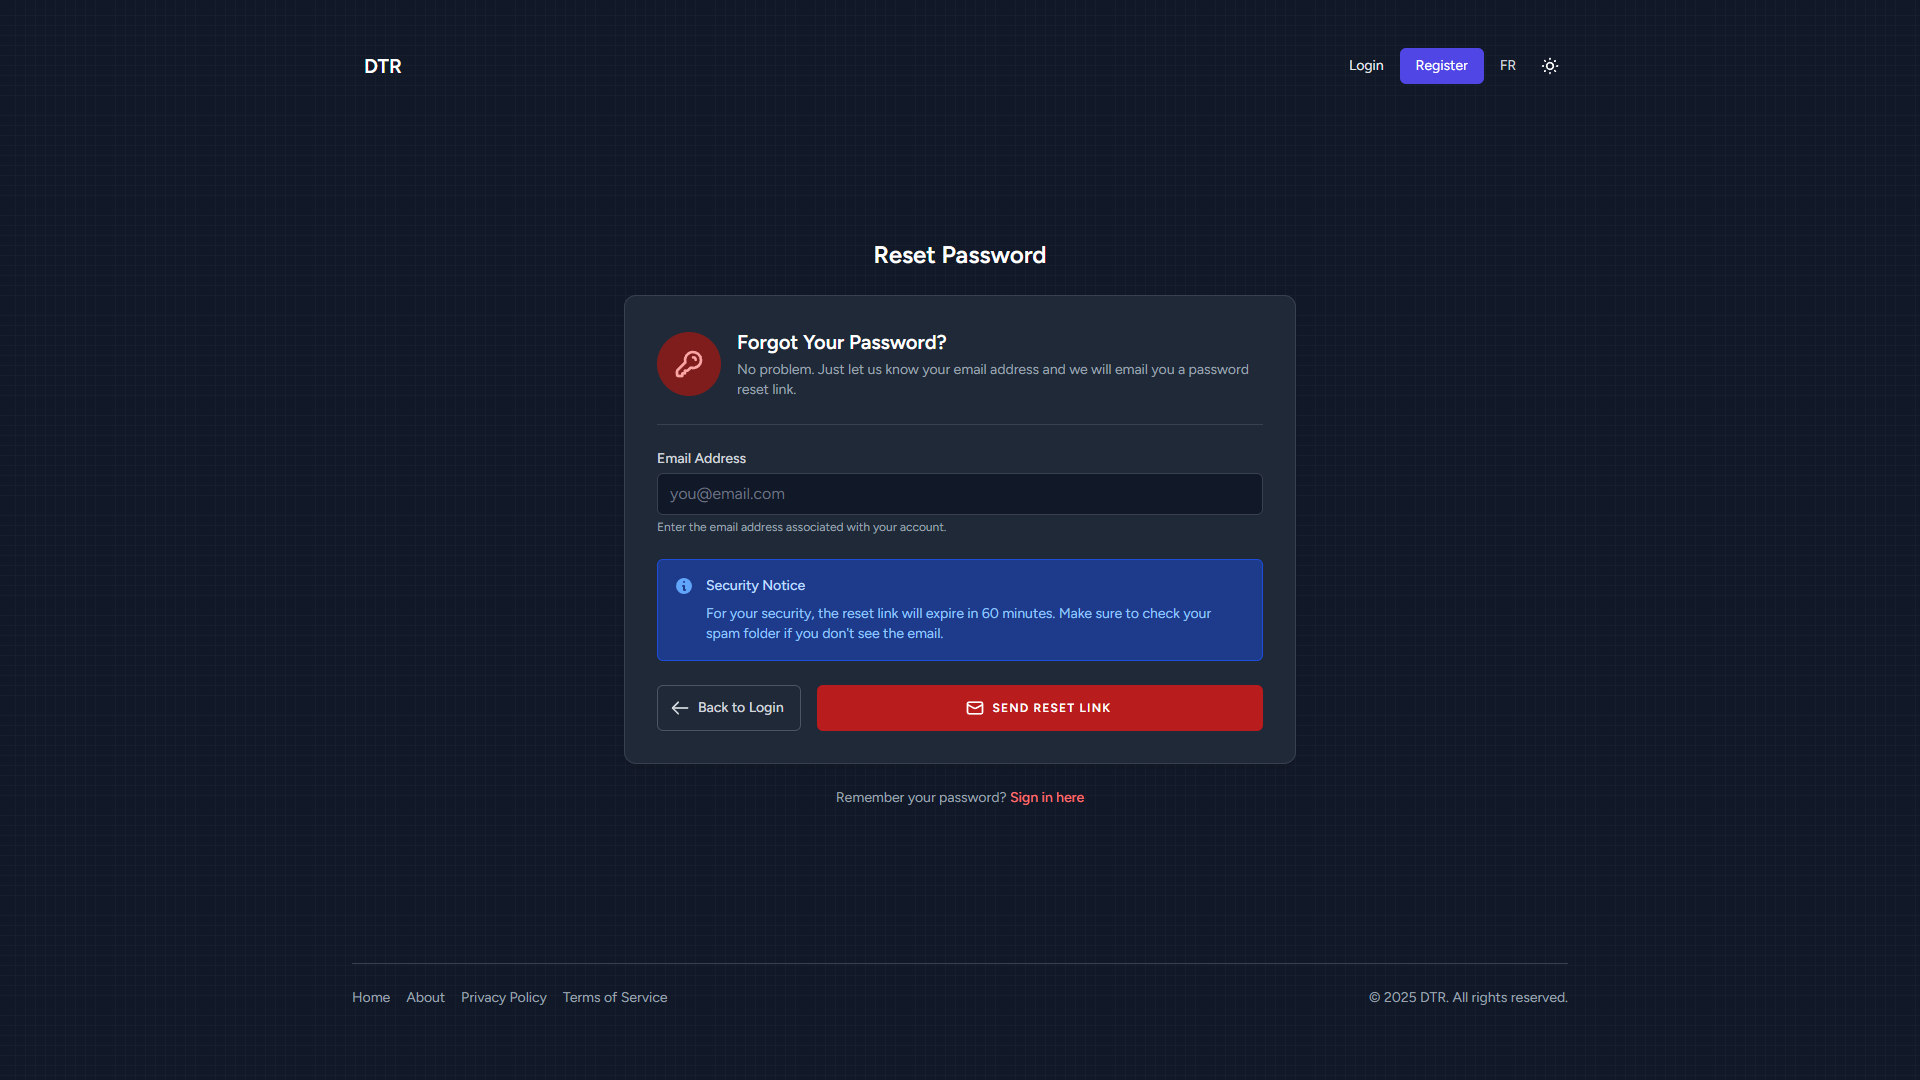
\includegraphics[width=0.85\textwidth]{assets/chapter4/screenshots/iotreap-landing-page.png}
\caption{IoT-REAP Landing Page}
\label{fig:landing-page}
\end{figure}

\subsection{Authentication System}

The authentication system was implemented using Laravel Fortify and integrated frontend pages. It provides the core security flows required by the platform, including account registration, login, password reset, email verification, and optional two-factor authentication. This subsystem ensures that only authenticated and verified users can access sensitive areas such as lab sessions, training progression, instructor tools, and administrative operations.

A notable aspect of the implementation is role-aware redirection. Once authenticated, users are directed to different areas according to their role and approval status. Teachers may be redirected to their teaching dashboard or to a pending approval page, administrators are redirected to administration interfaces, and engineers or learners access the operational dashboard and training interfaces relevant to their permissions.

The Google OAuth flow is managed by a dedicated GoogleOAuthService and a five-endpoint controller that handles the complete lifecycle: redirect to Google, handle the callback, present a role selection page for new users, process the selected role, and complete registration. After Google authentication, users who do not yet have a platform account are presented with an oauth-select-role page where they choose their intended role. The role-aware redirect logic then directs approved teachers to the teaching dashboard, pending teachers to an approval waiting page, administrators to the admin panel, and engineers or learners to their respective operational interfaces.

\begin{figure}[H]
\centering
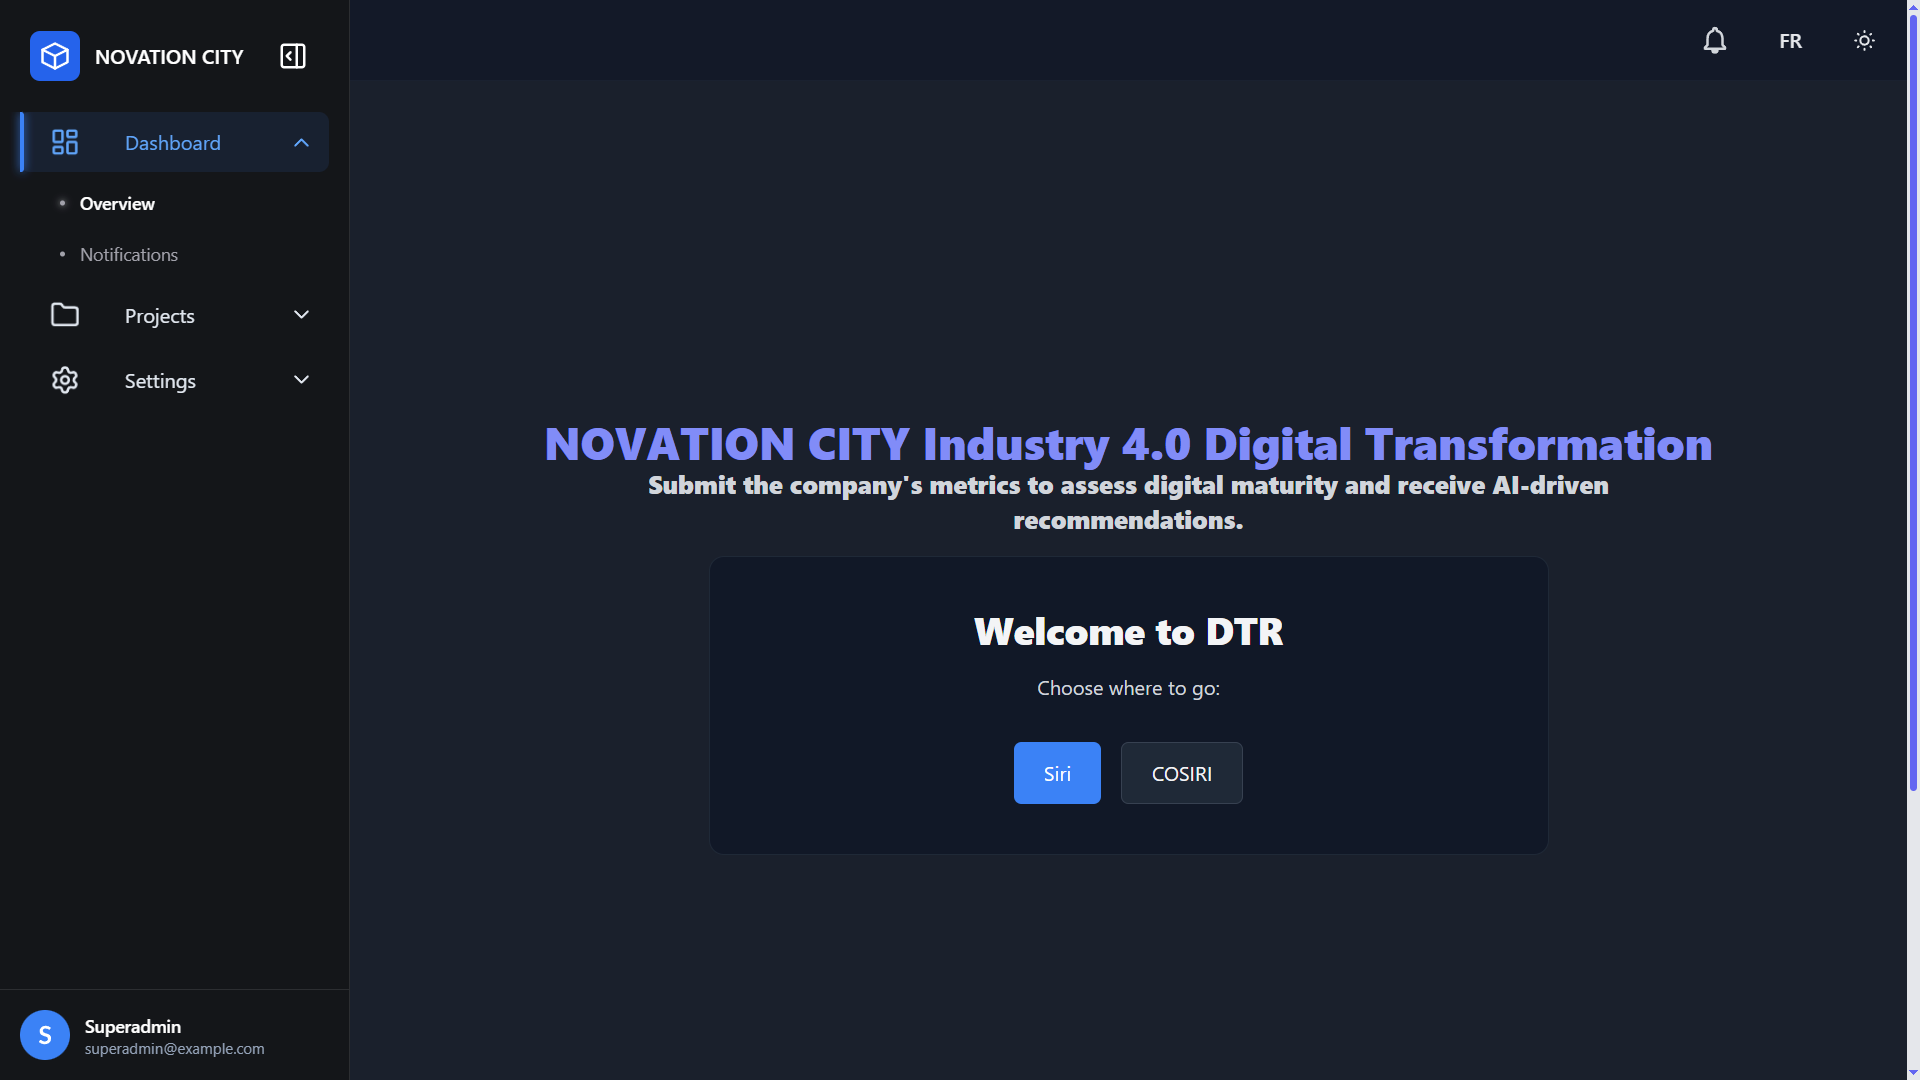
\includegraphics[width=0.85\textwidth]{assets/chapter4/screenshots/iotreap-login.png}
\caption{Authentication Login Interface}
\label{fig:login}
\end{figure}

\begin{figure}[H]
\centering
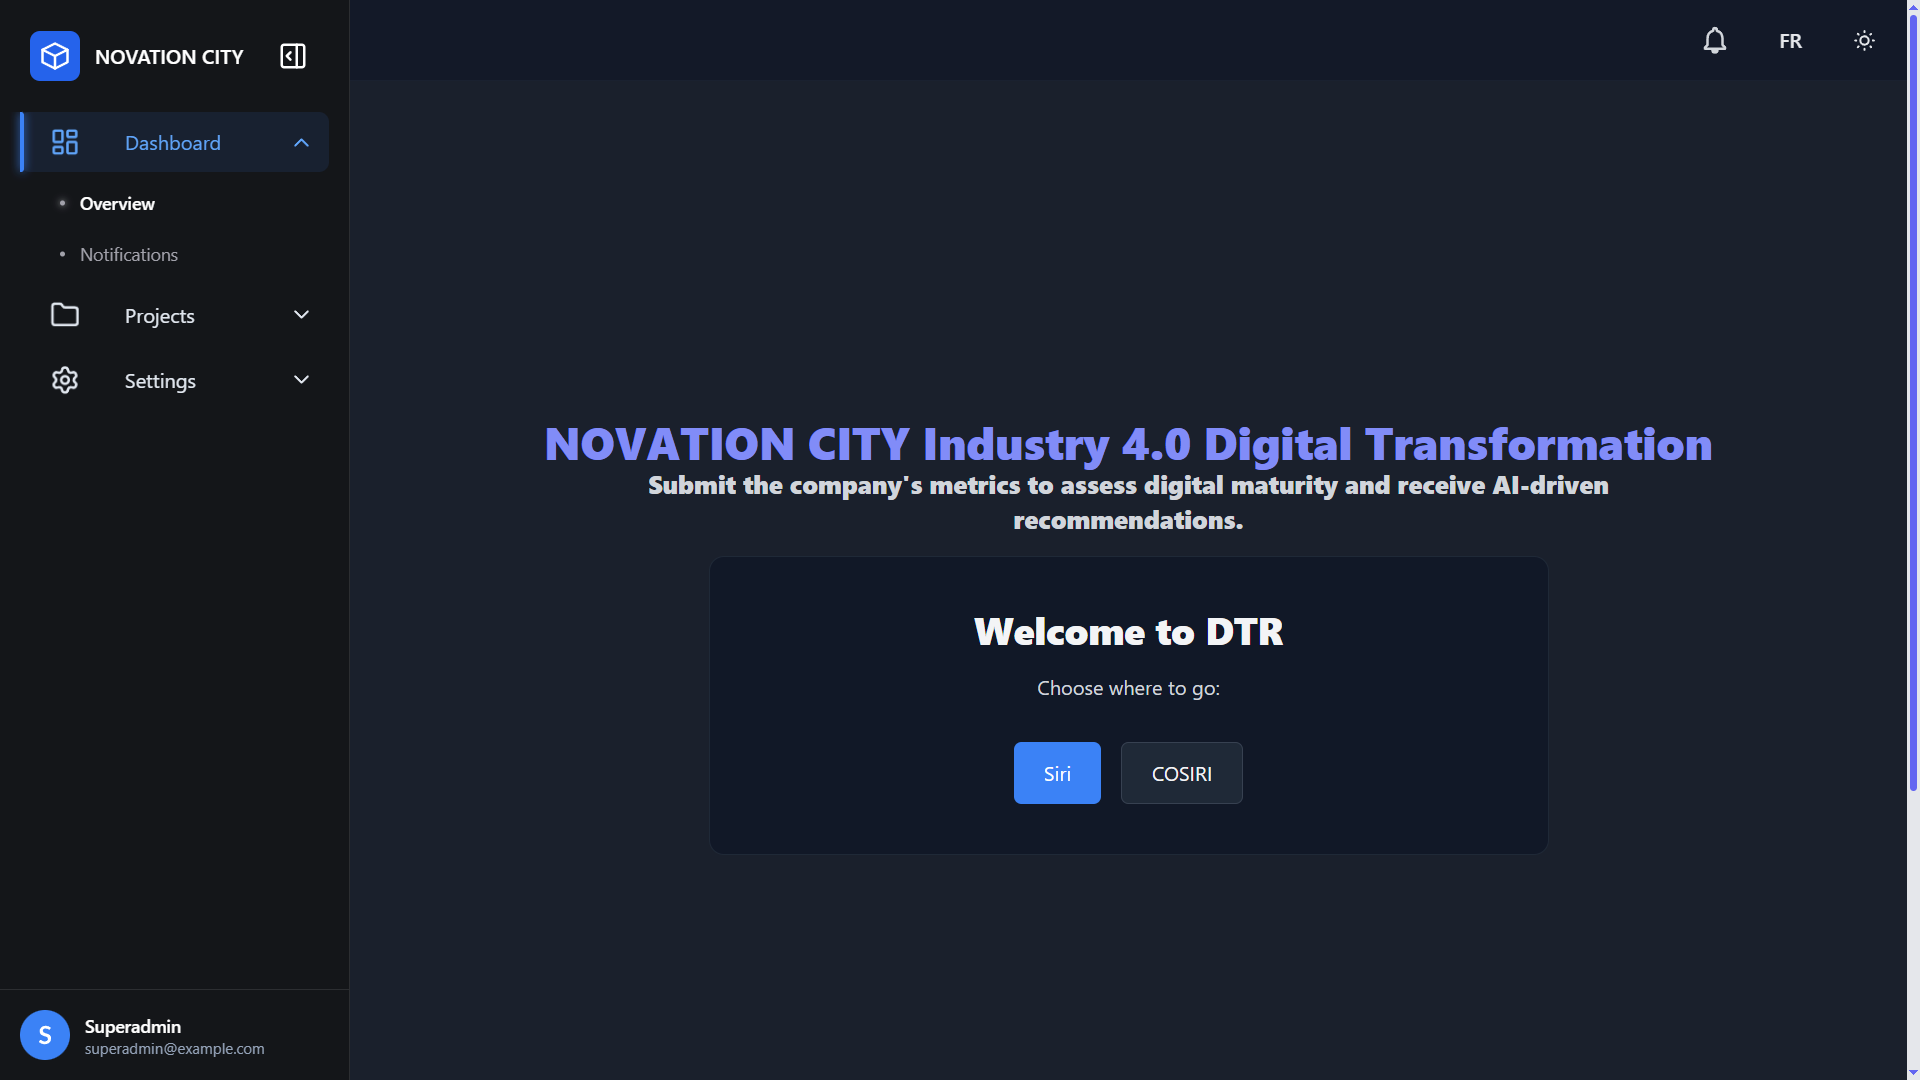
\includegraphics[width=0.85\textwidth]{assets/chapter4/screenshots/iotreap-register.png}
\caption{User Registration Interface with Role Selection}
\label{fig:register}
\end{figure}

\subsection{Operations Dashboard and VM Session Interfaces}

One of the central implementation goals of IoT-REAP is the delivery of browser-accessible operational sessions. For this reason, the platform includes a dedicated session management domain through which authorized users can browse available VM resources, provision sessions, extend active sessions, terminate them, and inspect remote access details.

The VM session module interacts with Proxmox-related services to coordinate virtual machine provisioning and with Guacamole-related services to generate browser-compatible remote access tokens. This design allows the user to access training or operational resources directly from the web application without installing a dedicated client. Additional configuration support is provided through connection preference management, allowing protocol-specific profiles and per-VM defaults to be stored. Connection preference management is implemented as a dedicated feature with its own page, controller, and two supporting models: GuacamoleConnectionPreference stores protocol-specific parameters such as color depth, resolution, and keyboard layout for RDP, VNC, and SSH protocols, while UserVMConnectionDefaultProfile stores per-VM default profiles that are automatically applied when a user connects to a specific session. Users configure these preferences through a dedicated interface accessible from the session view, and the settings are validated through dedicated FormRequest classes before being persisted.

The implementation also includes session-level resource interaction. Users can access session cameras, request control over available devices, change stream resolution, and manage hardware attachment flows. In this way, the session interface is not limited to remote desktop access; it becomes a unified work area for virtual and physical resource usage.

\begin{figure}[H]
\centering
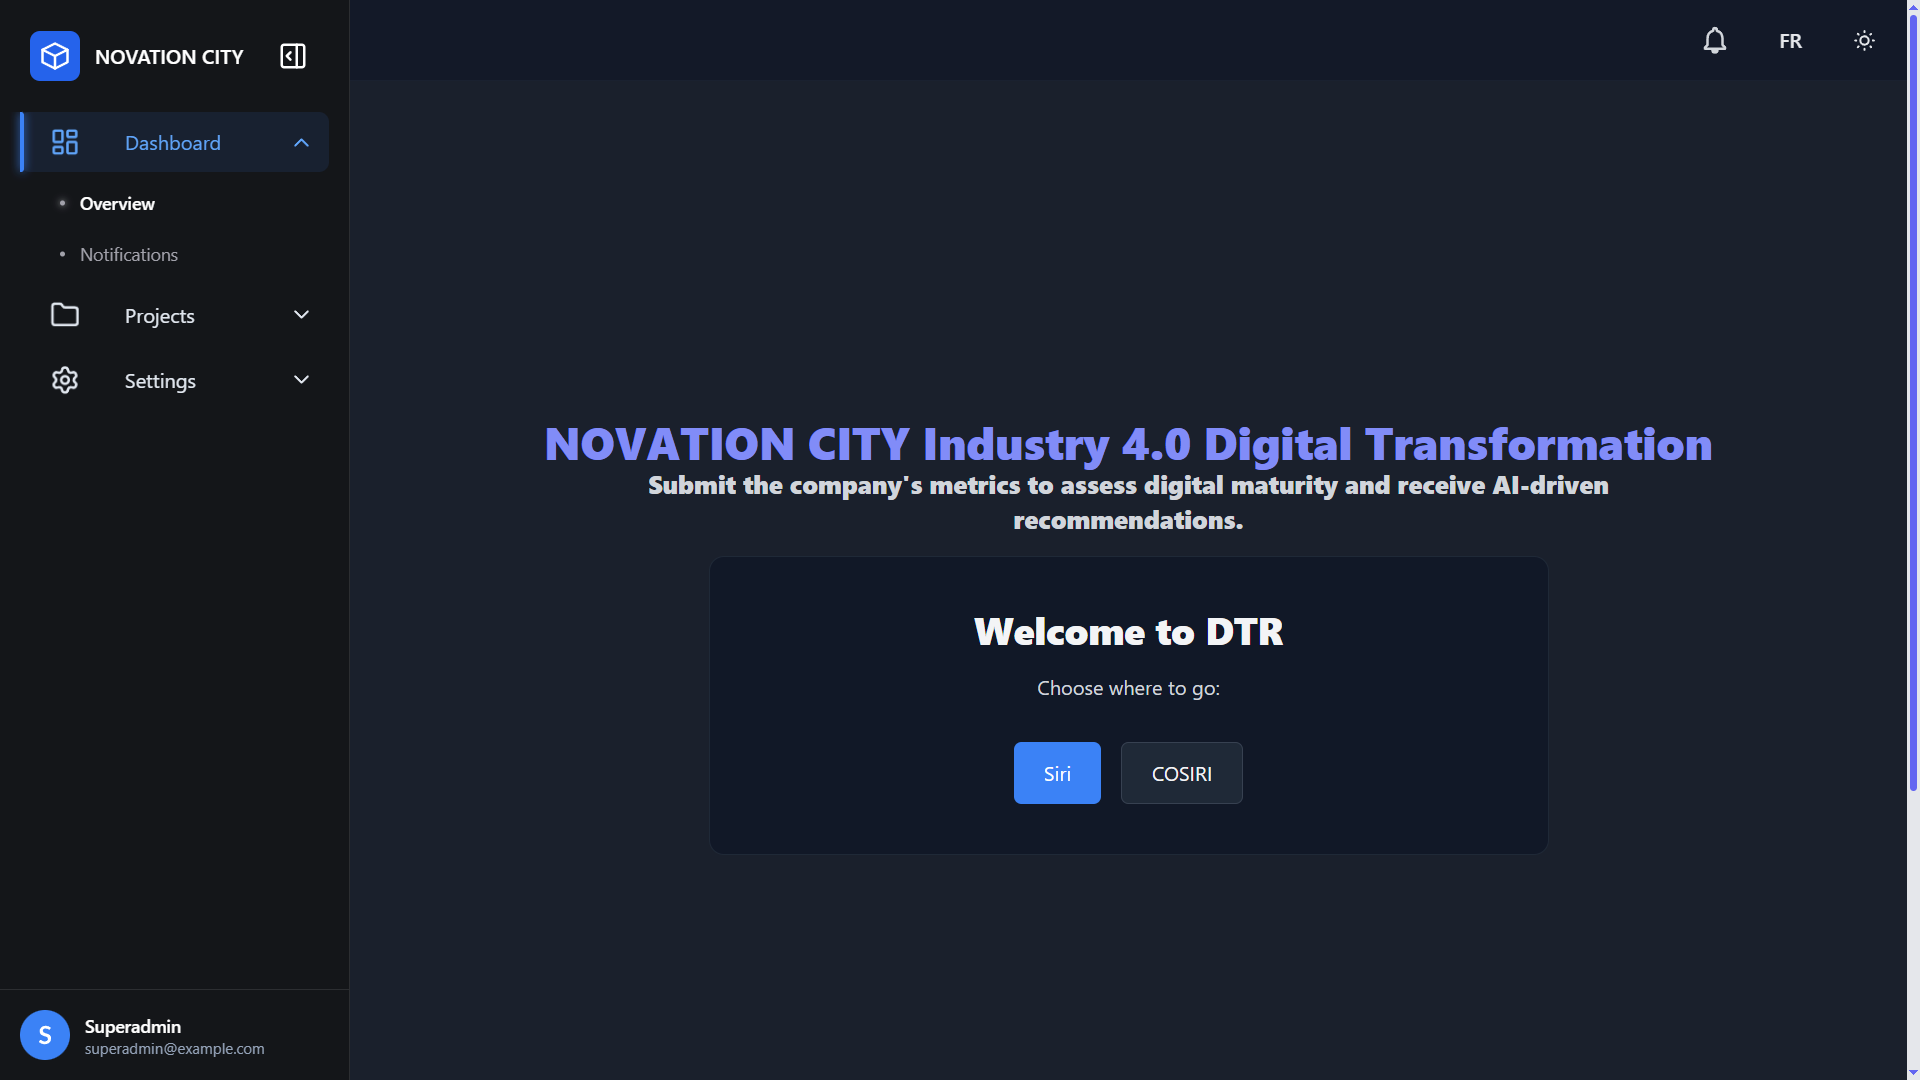
\includegraphics[width=0.85\textwidth]{assets/chapter4/screenshots/iotreap-vm-sessions.png}
\caption{VM Session Management and Remote Access Interface}
\label{fig:vm-sessions}
\end{figure}

The backend implementation of the VM session domain follows the platform's layered architecture. The VM session creation service receives validated input from the controller, persists the session record through the repository layer, and then delegates Guacamole connection setup to the Guacamole client service. The service logs each step of the process---session creation, connection establishment, and error conditions---to support operational monitoring and debugging. If the Guacamole connection fails, the exception is caught, logged with contextual details, and re-thrown so that the controller can return an appropriate error response.

The Guacamole client service handles the creation of browser-accessible remote desktop connections through the Guacamole HTTP API. It first obtains an authentication token from the Guacamole server, then separates connection parameters (such as hostname, port, and credentials) from connection attributes (such as maximum concurrent connections and failover settings). The service sends a structured request to the Guacamole API endpoint, including the connection name, protocol identifier, parent folder, parameters, and attributes. Upon success, the API returns a unique connection identifier that the service stores in the session record for later retrieval.

On the frontend, the VM session page uses a custom React hook that encapsulates all data fetching and session lifecycle actions. The hook manages three state variables: the list of active sessions, a loading indicator, and an error message. When the component mounts, the hook automatically fetches the user's sessions from the backend API. It also exposes functions for creating new sessions and terminating existing ones, both of which trigger a refresh of the session list after completion. This pattern ensures that the UI always reflects the latest session state without requiring manual data synchronization.

The API resource layer transforms Eloquent models into consistent JSON responses consumed by the React frontend. Each session resource includes the session identifier, current status, protocol type, connection profile name, VM identifier, node name, expiration timestamp, remaining time in seconds, IP address, Guacamole connection identifier, and the Guacamole access URL. When the user relationship is loaded, the resource also includes the user's identifier, name, and email. This structured response format ensures that the frontend receives only the data it needs, while internal fields such as Proxmox credentials and Guacamole tokens remain excluded.

The Proxmox integration includes a retry mechanism with exponential backoff: the provisioning service attempts the clone operation up to three times with increasing delays (2, 5, and 10 seconds), handling transient API failures gracefully. Template VMs are allocated from the VMID range 100--199, while session VMs receive identifiers from the range 200--999, preventing conflicts between templates and running instances. The ProxmoxLoadBalancer selects the target node using a weighted scoring algorithm that prioritizes available RAM at 70 percent weight over CPU utilization at 30 percent, with a load threshold of 85 percent to avoid overloading any single node. When a VM is first created, the ProxmoxIPResolver actively polls the guest agent for the assigned IP address, falling back to a static DHCP lease assignment if the agent does not respond within the timeout period.

Sessions support two operational modes: ephemeral sessions that are automatically destroyed upon expiration, and persistent sessions whose VMs are preserved for repeated access. Users can extend active sessions through the ExtendSessionService, and the VMReservationService allows advance booking of VM resources with conflict detection. The platform also supports VM snapshot operations---create, delete, and rollback---enabling users to save and restore VM states during practical exercises.

\subsection{Training Path Interfaces}

The training path module transforms IoT-REAP from a pure remote access platform into a complete technical learning environment. Public users can browse training paths, read details, inspect reviews, and search by category or keyword. Authenticated learners can enroll, access their personalized list of training paths, and continue their progression through assigned modules and training units.

From an implementation perspective, this module combines public catalog features with learner-specific progression tracking. The backend manages business rules related to enrollment, completion, review management, and note aggregation, while the frontend provides the structured navigation and responsive display needed for an educational workflow.

\begin{figure}[H]
\centering
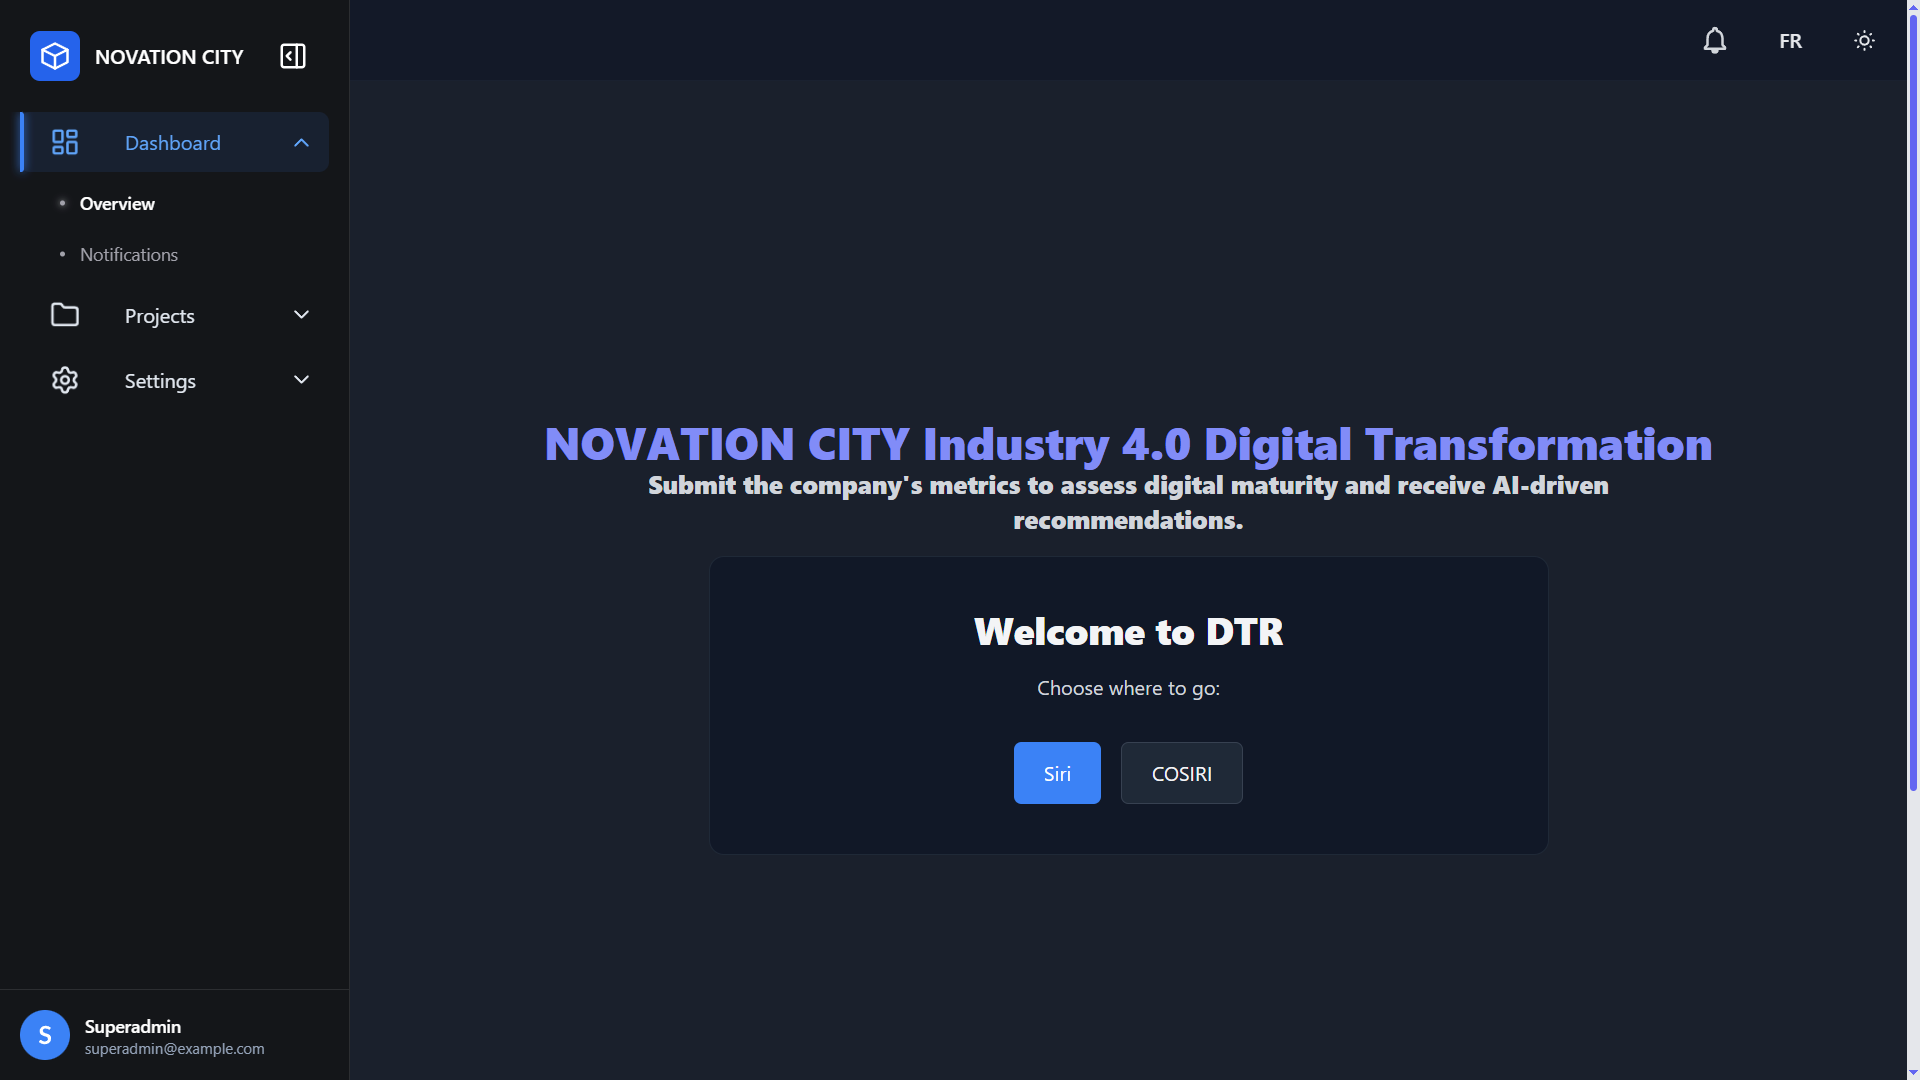
\includegraphics[width=0.85\textwidth]{assets/chapter4/screenshots/iotreap-training-paths.png}
\caption{Training Path Catalog and Learner Progression Interface}
\label{fig:training-paths}
\end{figure}

\subsection{Training Unit Learning Interface}

The training unit interface is the operational center of the learner experience. Each training unit can be associated with different instructional media and practical resources such as videos, reading articles, quizzes, notes, and VM-based activities. This design supports blended learning, where theoretical content and practical execution coexist within the same structured path.

Video-oriented units support streaming and progress tracking, article units support reading completion, quiz units support attempt management and grading history, and VM-enabled units can be linked to remote lab resources. This implementation directly supports the pedagogical objective established in the previous chapters: enabling technical upskilling through guided learning combined with hands-on practice.

\begin{figure}[H]
\centering
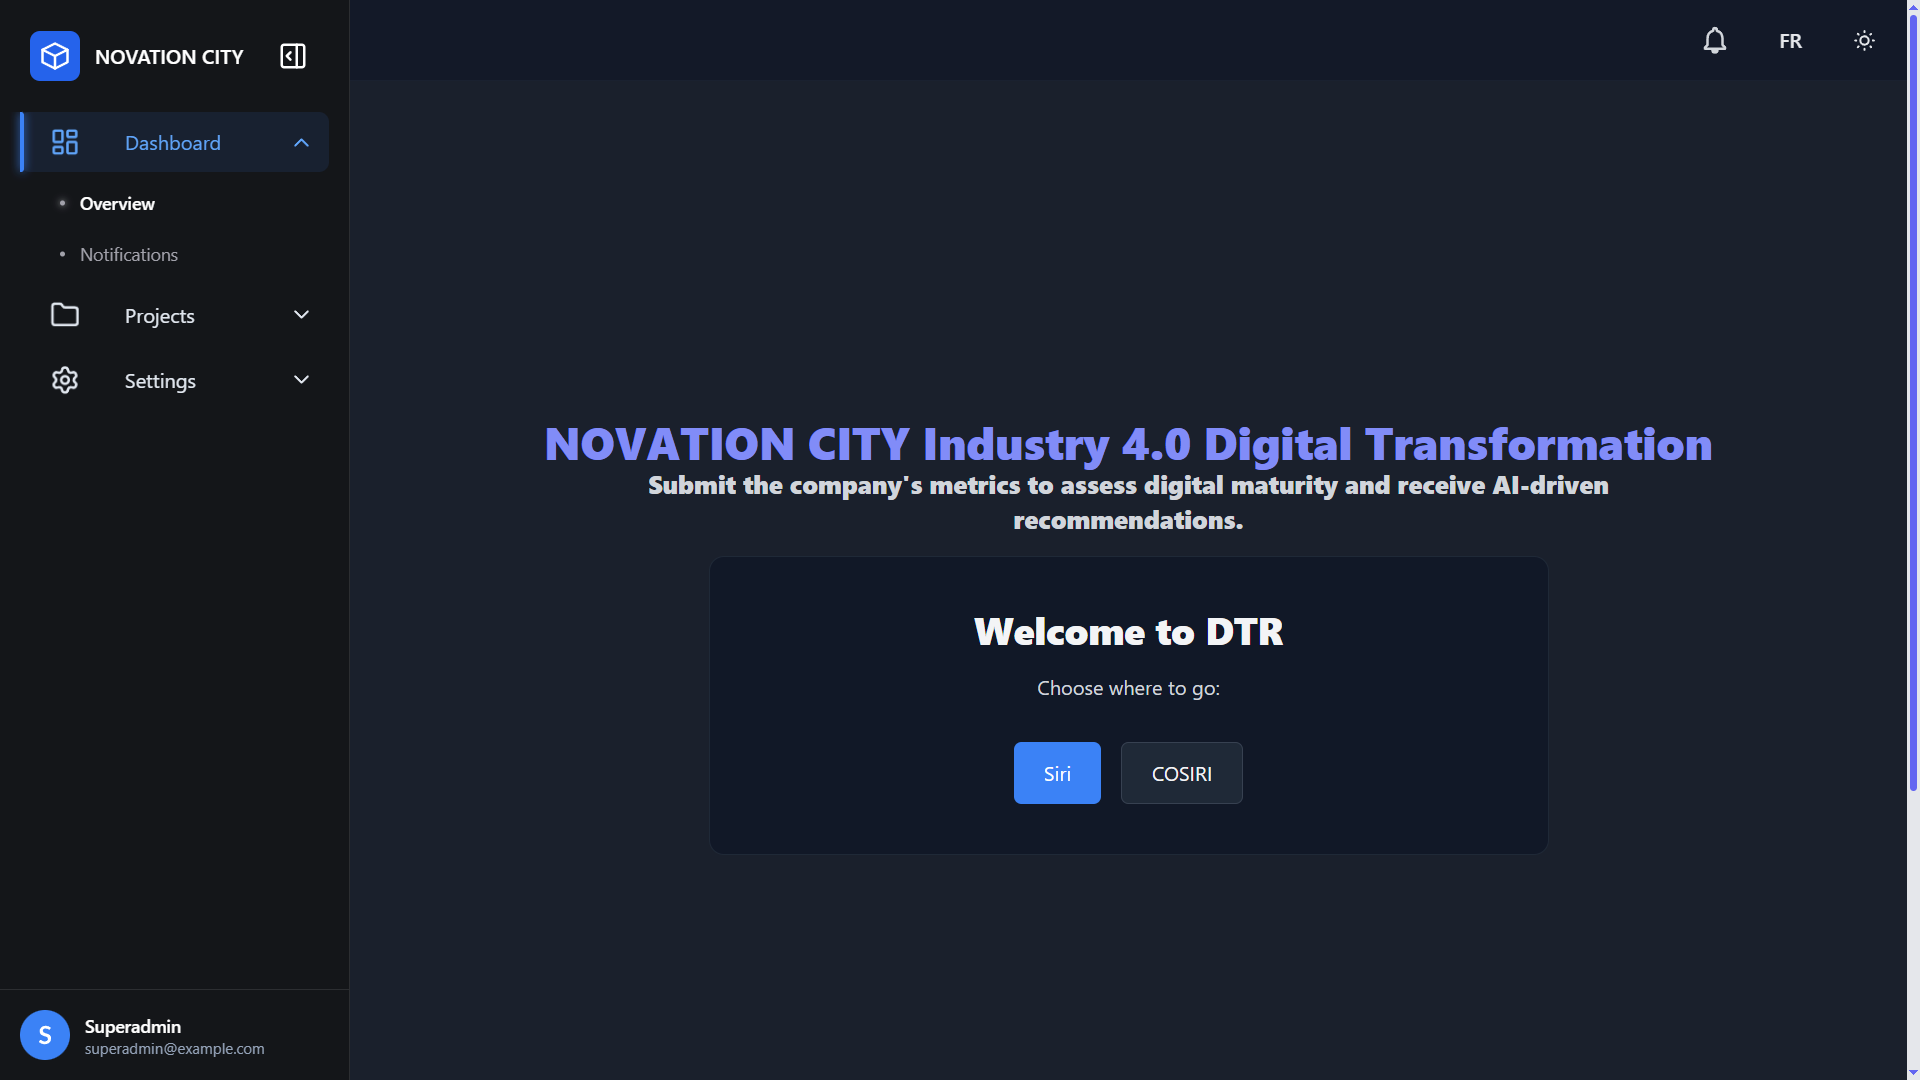
\includegraphics[width=0.85\textwidth]{assets/chapter4/screenshots/iotreap-training-unit.png}
\caption{Training Unit Learning Interface with Blended Content}
\label{fig:training-unit}
\end{figure}

\subsection{Teaching Interfaces}

IoT-REAP includes a complete teaching area for instructors responsible for creating and maintaining technical content. The teaching module allows instructors to create training paths, update path metadata, define modules, create and reorder training units, and submit completed content for administrative review. This authoring workflow makes the platform extensible and enables internal growth of the training catalog.

The implementation goes further by providing specialized content editors for quizzes, articles, and videos. Instructors can configure quiz questions, publish or unpublish assessments, upload or manage training videos, maintain captions, and edit article-based lesson content. In addition, the platform includes instructor analytics, learner progress monitoring, earnings visualization, payout requests, and a forum inbox for handling learner interactions. This makes the teaching area not only a content management space but also an operational dashboard for pedagogical supervision.

\begin{figure}[H]
\centering
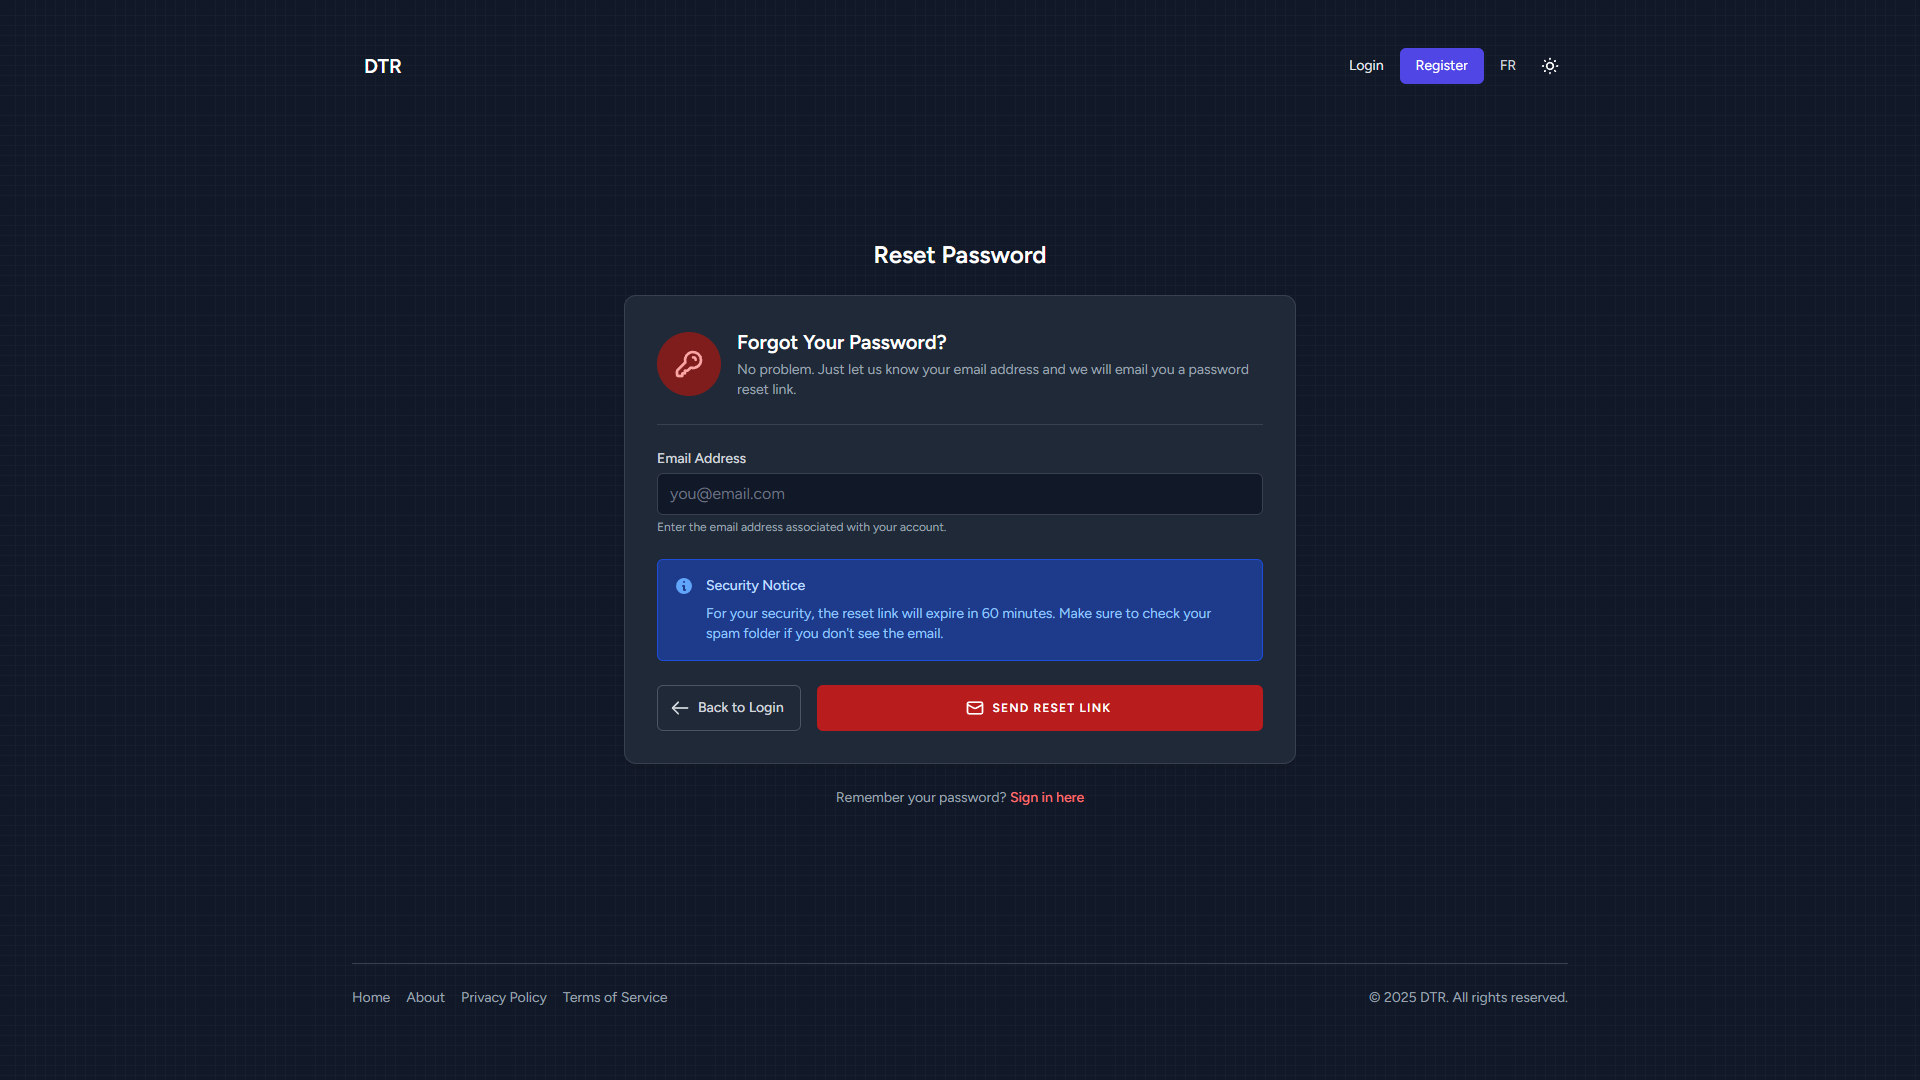
\includegraphics[width=0.85\textwidth]{assets/chapter4/screenshots/iotreap-teaching-dashboard.png}
\caption{Instructor Teaching Dashboard and Content Authoring Interface}
\label{fig:teaching-dashboard}
\end{figure}

\subsection{Administrative Interfaces}

The administrative domain is one of the broadest implementation areas of the platform. It supports governance of infrastructure, users, content approval, reservation workflows, financial operations, and operational supervision. Administrators can access a central dashboard with analytics and health indicators, manage infrastructure records, inspect nodes and virtual machines, configure Proxmox server records, and oversee hardware and maintenance states.

The administrative features also include user management with approval, suspension, role updates, impersonation, and privacy-related deletion actions. Content governance is supported through training path approval and featuring workflows. Operational control includes reservation review, camera assignment and reservation management, refund handling, payout processing, alert monitoring, activity logging, and moderation of flagged forum content.

This breadth of implementation reflects the dual nature of IoT-REAP: it is simultaneously a learning management platform and an operational orchestration system for remote industrial training resources.

Operational auditability is supported through an ActivityLogService that records significant platform events---such as user approvals, role changes, content publications, and administrative actions---in a persistent activity log. Administrators can query and filter this log through a dedicated controller, providing a traceable record of governance actions. The platform also maintains a SystemAlert model and associated AdminAlertService and SystemHealthService that track infrastructure health indicators, VM provisioning failures, and operational anomalies. Alerts are displayed on the administrative dashboard and can trigger notifications to responsible administrators.

\begin{figure}[H]
\centering
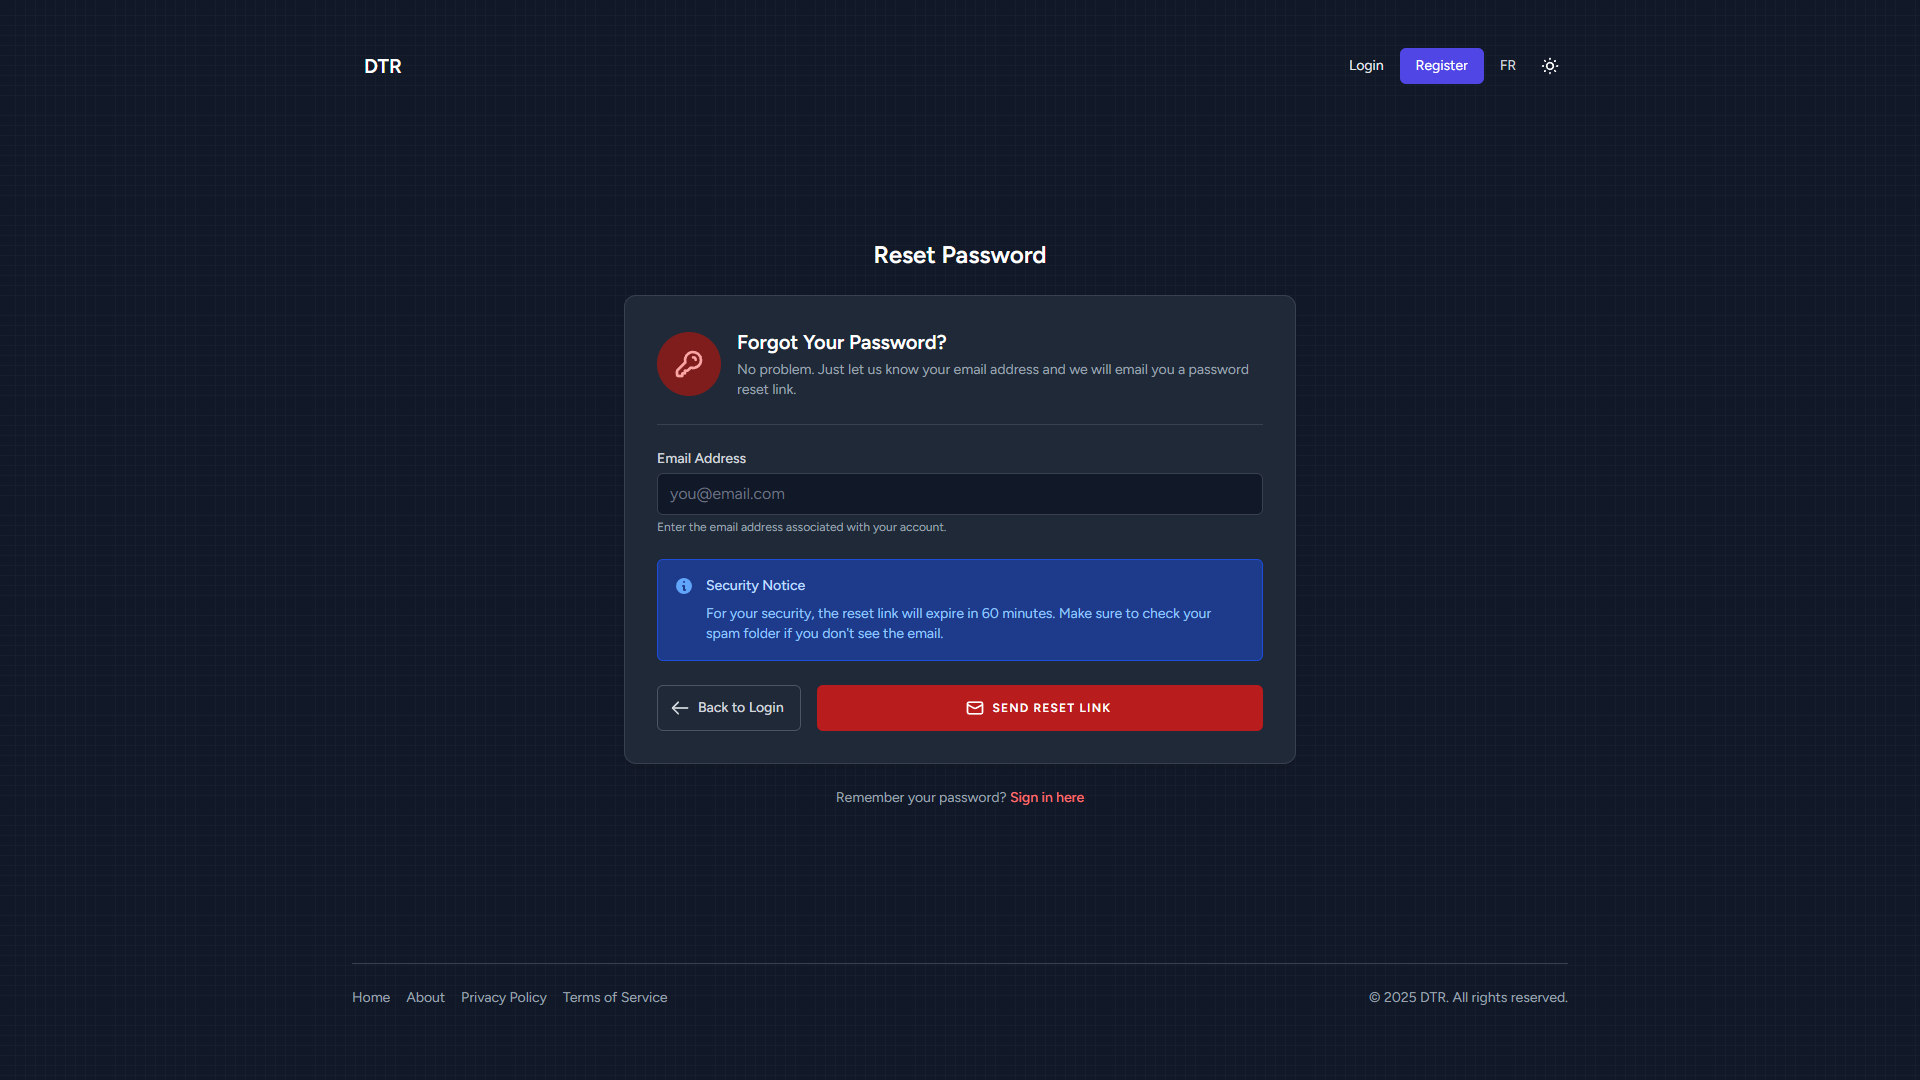
\includegraphics[width=0.85\textwidth]{assets/chapter4/screenshots/iotreap-admin-dashboard.png}
\caption{Administrative Dashboard and Infrastructure Governance Interface}
\label{fig:admin-dashboard}
\end{figure}

\subsection{Notifications, Certificates, Payments, and Reservations}

Several cross-cutting features complete the functional landscape of the platform. These areas—notifications, certificate generation and verification, payment and checkout, and reservation management—are described in the following dedicated subsections. Each subsection below provides the implementation details and operational considerations for that specific cross-cutting concern.

\subsection{Forum and Learner Interaction}
To support collaborative learning, IoT-REAP integrates a forum module where users can view, create, reply to, and interact with discussion threads attached either to training paths or to individual training units. This feature encourages peer assistance, content clarification, and knowledge sharing around technical training materials.

The implementation includes user interaction features such as upvoting, flagging, and reply management, while moderators and instructors receive additional controls for pinning threads, locking discussions, resolving flags, and marking helpful answers. This makes the forum both a learning tool and a moderated support space.

\subsection{Camera and Robotics Interface}

The camera and robotics interface is a distinctive feature of IoT-REAP that connects the web platform to the physical world of industrial and IoT equipment. This module provides browser-based access to live camera streams from operational environments and allows authorized users to issue remote commands to connected robots and devices.

From the backend perspective, camera management is handled through dedicated services that register camera devices, assign them to infrastructure nodes, and manage their availability for reservation. The streaming pipeline uses a WHEP (WebRTC-HTTP Egress Protocol) proxy for browser-compatible live stream delivery, with FFmpeg handling format adaptation and transcoding when required for browser playback.

Camera pan-tilt-zoom (PTZ) operations are protected by an exclusive lock mechanism: only one user may hold the PTZ lock for a given camera at a time, preventing conflicting control commands from multiple simultaneous users. Camera visibility is scoped to the user's role and session context---engineers can only view and control cameras assigned to their active sessions, while administrators have global visibility. The platform supports multiple camera types including fixed IP cameras, PTZ-capable cameras, and USB cameras attached through gateway nodes, each with type-specific configuration parameters stored in the database.

The robotics command interface uses MQTT as the communication protocol. Robot commands are published to topic-based channels following a robot-specific command topic format with QoS\,1 delivery guarantees, ensuring that operational instructions reach their target devices reliably. Telemetry data flows in the opposite direction, with devices publishing to a robot-specific telemetry topic and the platform subscribing to receive status updates. This bidirectional communication model enables real-time remote operation of industrial equipment from within the browser.

The MQTT service implementation demonstrates how the platform publishes robot commands with QoS\,1 delivery. The service constructs the topic by replacing a placeholder in the configured topic pattern with the target robot identifier, then assembles a structured payload containing the action type, parameters, and a timestamp. The publish method first attempts delivery through an HTTP bridge to the gateway agent, which provides a reliable and centrally managed publishing path. If the HTTP bridge is unavailable---for example, due to a network timeout---the service logs a warning and falls back to direct CLI-based publishing. This dual-path approach ensures that robot commands are delivered even when the preferred bridge mechanism is temporarily unreachable.

\begin{figure}[H]
\centering
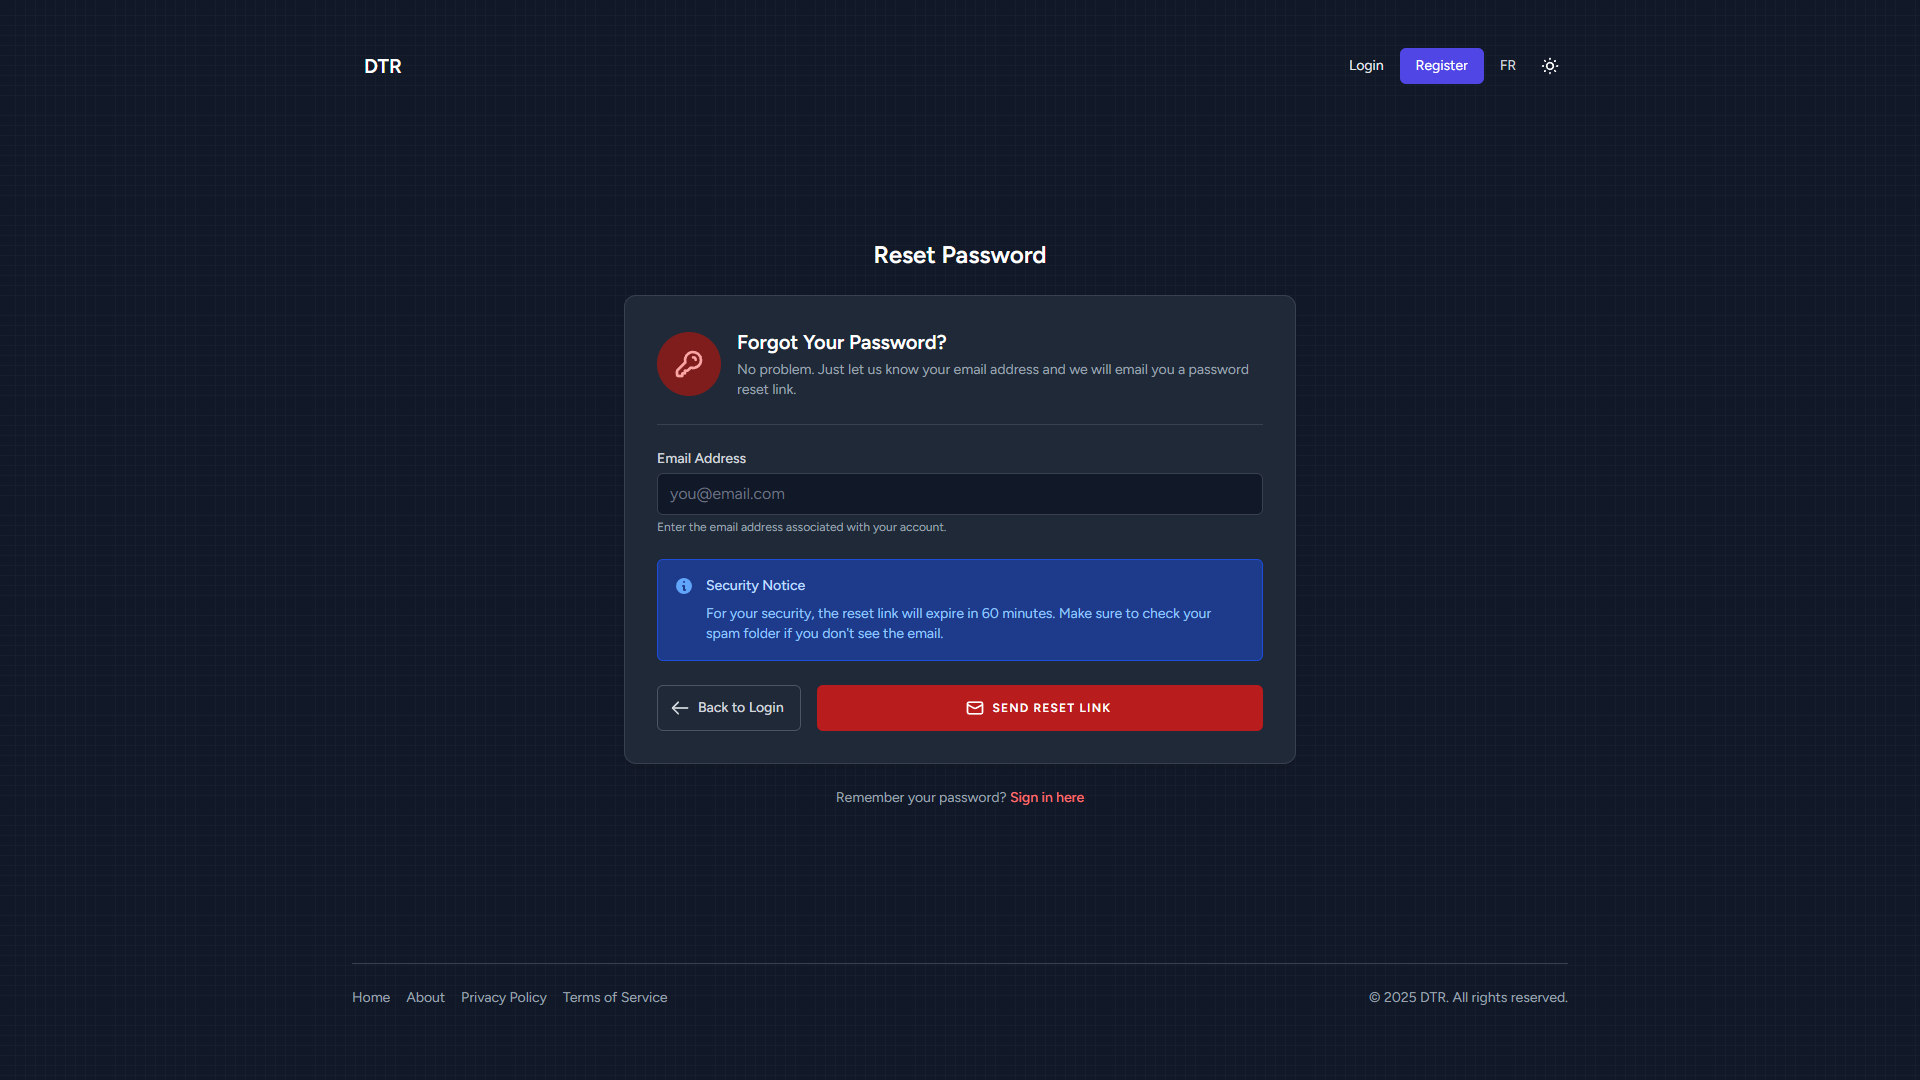
\includegraphics[width=0.85\textwidth]{assets/chapter4/screenshots/iotreap-camera-robotics.png}
\caption{Camera and Robotics Control Interface}
\label{fig:camera-robotics}
\end{figure}

\subsection{Hardware and USB/IP Interface}

The hardware and USB/IP interface extends IoT-REAP's remote access capabilities beyond virtual machines to physical USB devices attached to gateway nodes. This module enables authorized engineers to attach remote USB devices---such as cameras, serial adapters, or programming tools---to their active VM sessions over IP, effectively providing the same experience as if the device were physically plugged into their local machine.

The implementation relies on USB/IP protocol services running on gateway nodes, managed through a dedicated backend service that tracks available devices, their connection states, and their assignment to active sessions. When a user requests a USB device attachment, the platform coordinates the USB/IP binding on the target gateway node and updates the session record to reflect the hardware state. Device detachment and cleanup are handled automatically when sessions expire or are terminated, preventing orphaned device locks.

Administrators can manage the hardware inventory, register new USB devices, assign them to specific gateway nodes, and monitor their utilization across sessions. This interface is essential for scenarios where engineers need to interact with physical training equipment---such as microcontrollers, PLCs, or industrial sensors---during remote lab sessions.

The USB attachment workflow uses a queued job system to handle the potentially slow USB/IP binding process asynchronously. Device paths on Windows gateway nodes are resolved using DOS 8.3 short-name format to avoid issues with spaces and special characters in USB device paths. An auto-reattach mechanism monitors active sessions and reattaches USB devices that were previously bound if the VM is restarted or migrated. A reconcile artisan command is also available to scan all gateway nodes, compare reported USB devices against the database inventory, and correct any drift between the actual hardware state and the recorded state.

\begin{figure}[H]
\centering
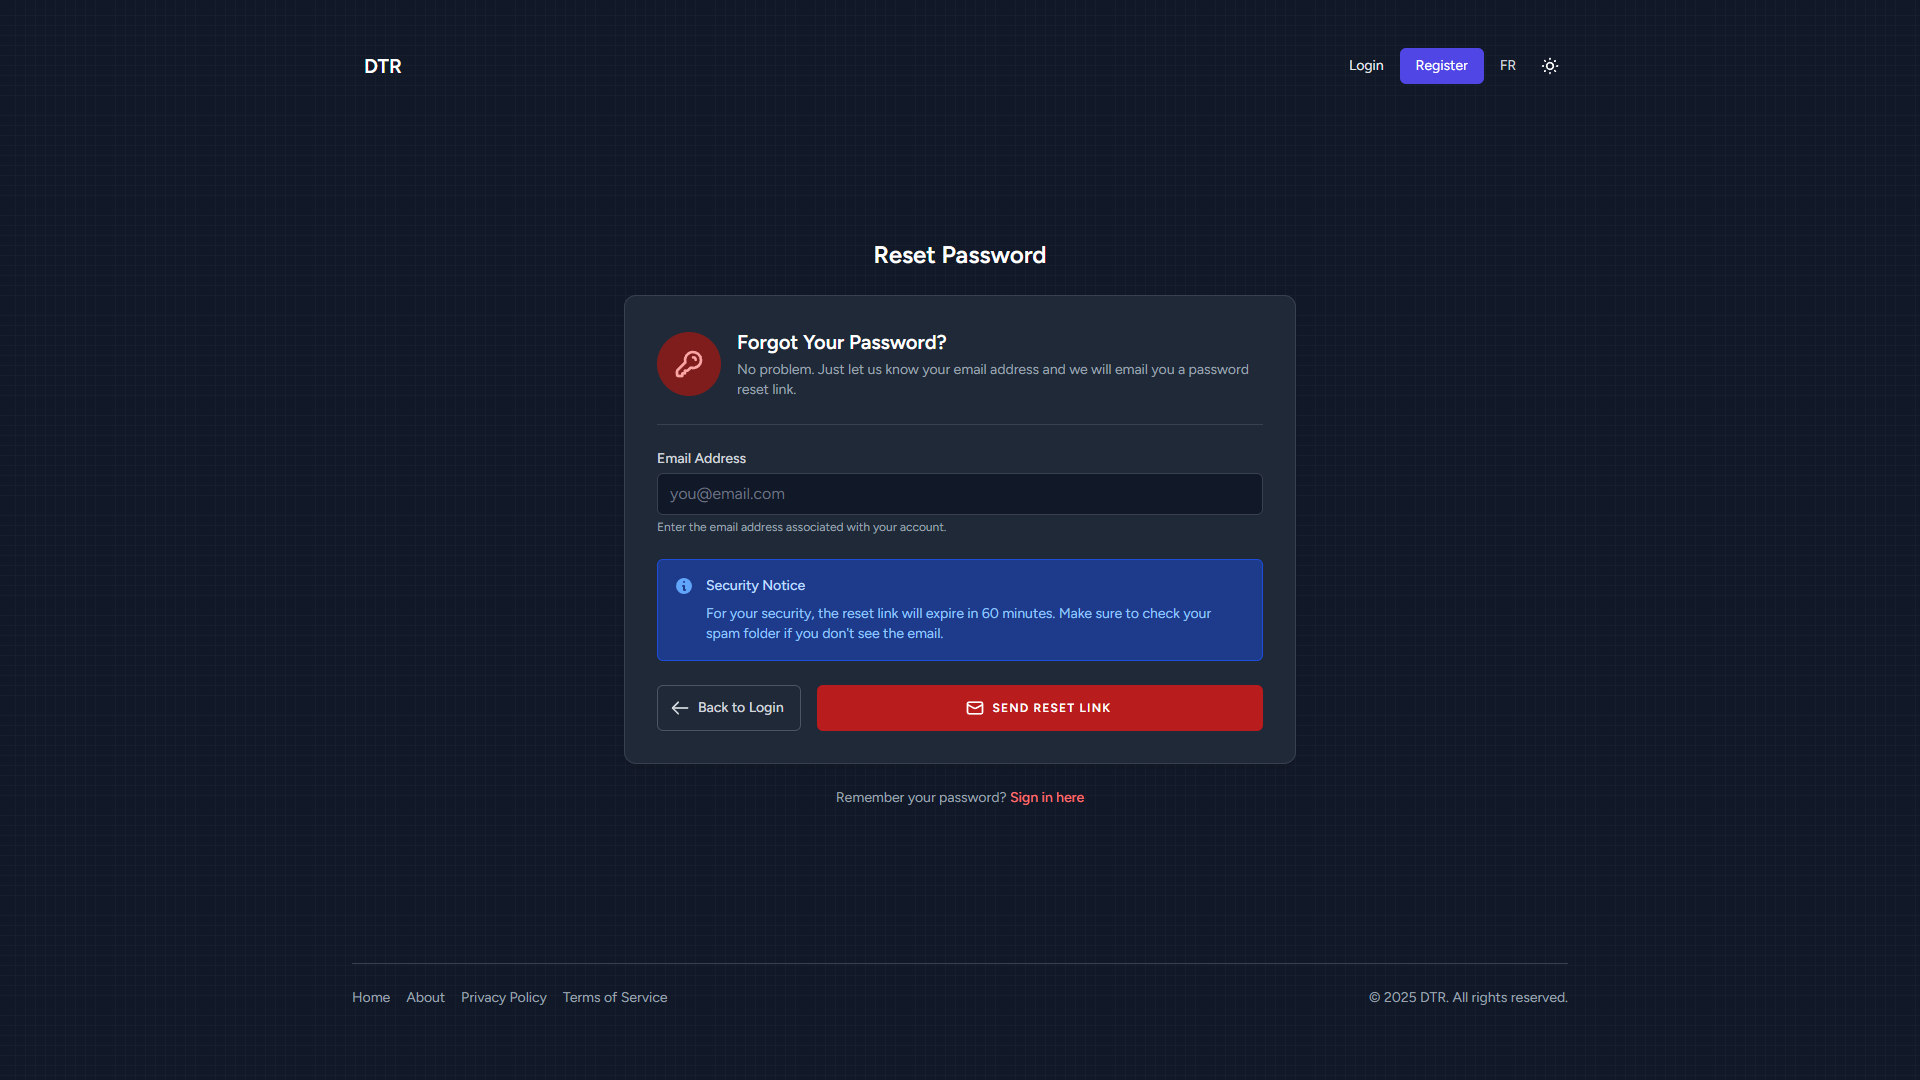
\includegraphics[width=0.85\textwidth]{assets/chapter4/screenshots/iotreap-hardware-usb.png}
\caption{Hardware and USB/IP Device Management Interface}
\label{fig:hardware-usb}
\end{figure}

\subsection{Search and Discovery Interface}

The search and discovery module provides users with efficient ways to find training paths, training units, and other platform content. The implementation supports keyword-based search with filtering by category, difficulty level, and content type, enabling learners and visitors to quickly locate relevant educational resources.

From the backend, search queries are processed through a dedicated SearchRepository that applies scoped queries against training path and training unit records, with the SearchService coordinating query construction and result ranking. The frontend exposes the search interface through a GlobalSearch component that provides a command-palette-style interface with instant results, category badges, and direct navigation links. This module is particularly important for platforms with growing catalogs, where manual browsing alone would be insufficient for content discovery.

\begin{figure}[H]
\centering
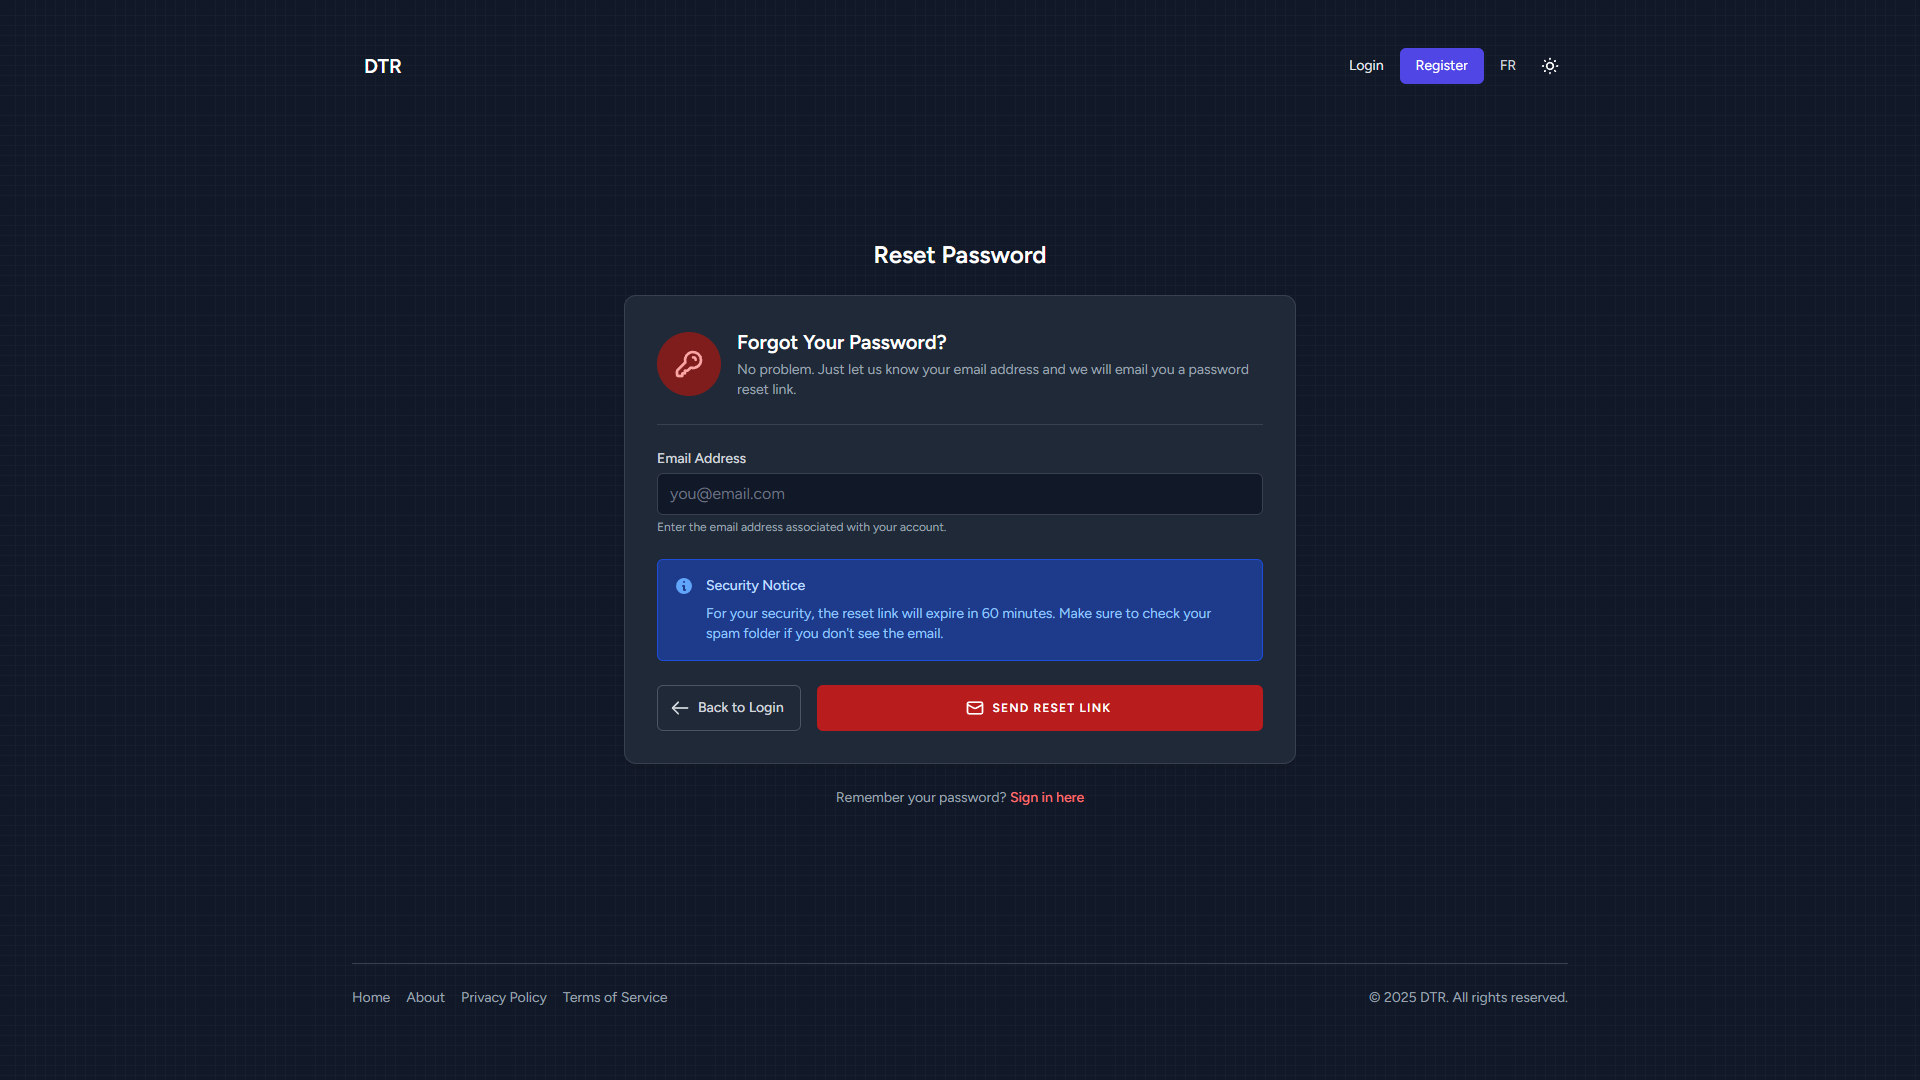
\includegraphics[width=0.85\textwidth]{assets/chapter4/screenshots/iotreap-search-results.png}
\caption{Search and Discovery Results Interface}
\label{fig:search-discovery}
\end{figure}

\subsection{Video Streaming Interface}

The video streaming interface supports the delivery of instructional video content within training units. Unlike the live camera streams described earlier, this module focuses on pre-recorded educational videos that instructors upload and manage as part of their teaching content.

The implementation handles video upload, storage, transcoding, and progressive delivery. Uploaded videos are processed through FFmpeg for format normalization and HLS segment generation, enabling adaptive bitrate streaming across different network conditions. The frontend player supports playback controls, progress tracking, and completion reporting, which feeds back into the learner's training unit progression state.

Instructors can manage their video library, update captions, replace source files, and control publication status. The video module integrates with the broader training unit system, ensuring that video-based lessons are tracked consistently alongside other content types such as quizzes and articles.

The transcoding pipeline generates three adaptive quality profiles: 360p at 800 kbps for low-bandwidth conditions, 720p at 2500 kbps for standard connections, and 1080p at 5000 kbps for high-fidelity playback. HLS segments are produced at 10-second intervals, and a thumbnail is automatically extracted at the 5-second mark at 640 by 360 resolution. The VideoService supports three execution modes for FFmpeg: auto mode, which attempts gateway-based transcoding via SSH and falls back to local execution if the gateway is unavailable; gateway-only mode, which requires a gateway node; and local-only mode, which runs FFmpeg directly on the application server. Transcoding and thumbnail generation are dispatched as asynchronous queue jobs---TranscodeVideoJob and GenerateThumbnailJob---to avoid blocking the request cycle. The VideoProgressService tracks each learner's playback position, enabling resume-from-last-position behavior across sessions.

\begin{figure}[H]
\caption{Video Streaming Player within a Training Unit}
\label{fig:video-player}
\end{figure}

\subsection{Quiz Engine Interface}

The quiz engine is a specialized content module that supports the creation, delivery, and evaluation of assessments within training units. Instructors can define quizzes with multiple question types, configure attempt limits and time constraints, and review grading results. Learners interact with the quiz engine to attempt assessments, view their scores, and review their answer history.

The backend implementation manages quiz lifecycle states (draft, published, closed), question ordering, answer validation, and score calculation. The quiz engine also supports automatic grading for objective question types and provides instructors with analytics on question difficulty and learner performance distribution. This module is tightly integrated with the training unit progression system, ensuring that quiz completion contributes to the learner's overall advancement.

Question types are governed by a QuizQuestionType enum that defines the supported formats: multiple-choice, true/false, and short-answer. Each quiz attempt is tracked through a QuizAttempt model that records the learner's answers, score, and timestamp, enabling both the learner and instructor to review historical performance. On the frontend, the quiz experience is delivered through dedicated React components for quiz attempt rendering, a quiz builder interface for instructors, and a results review page that displays per-question scoring and feedback.

\begin{figure}[H]
\centering
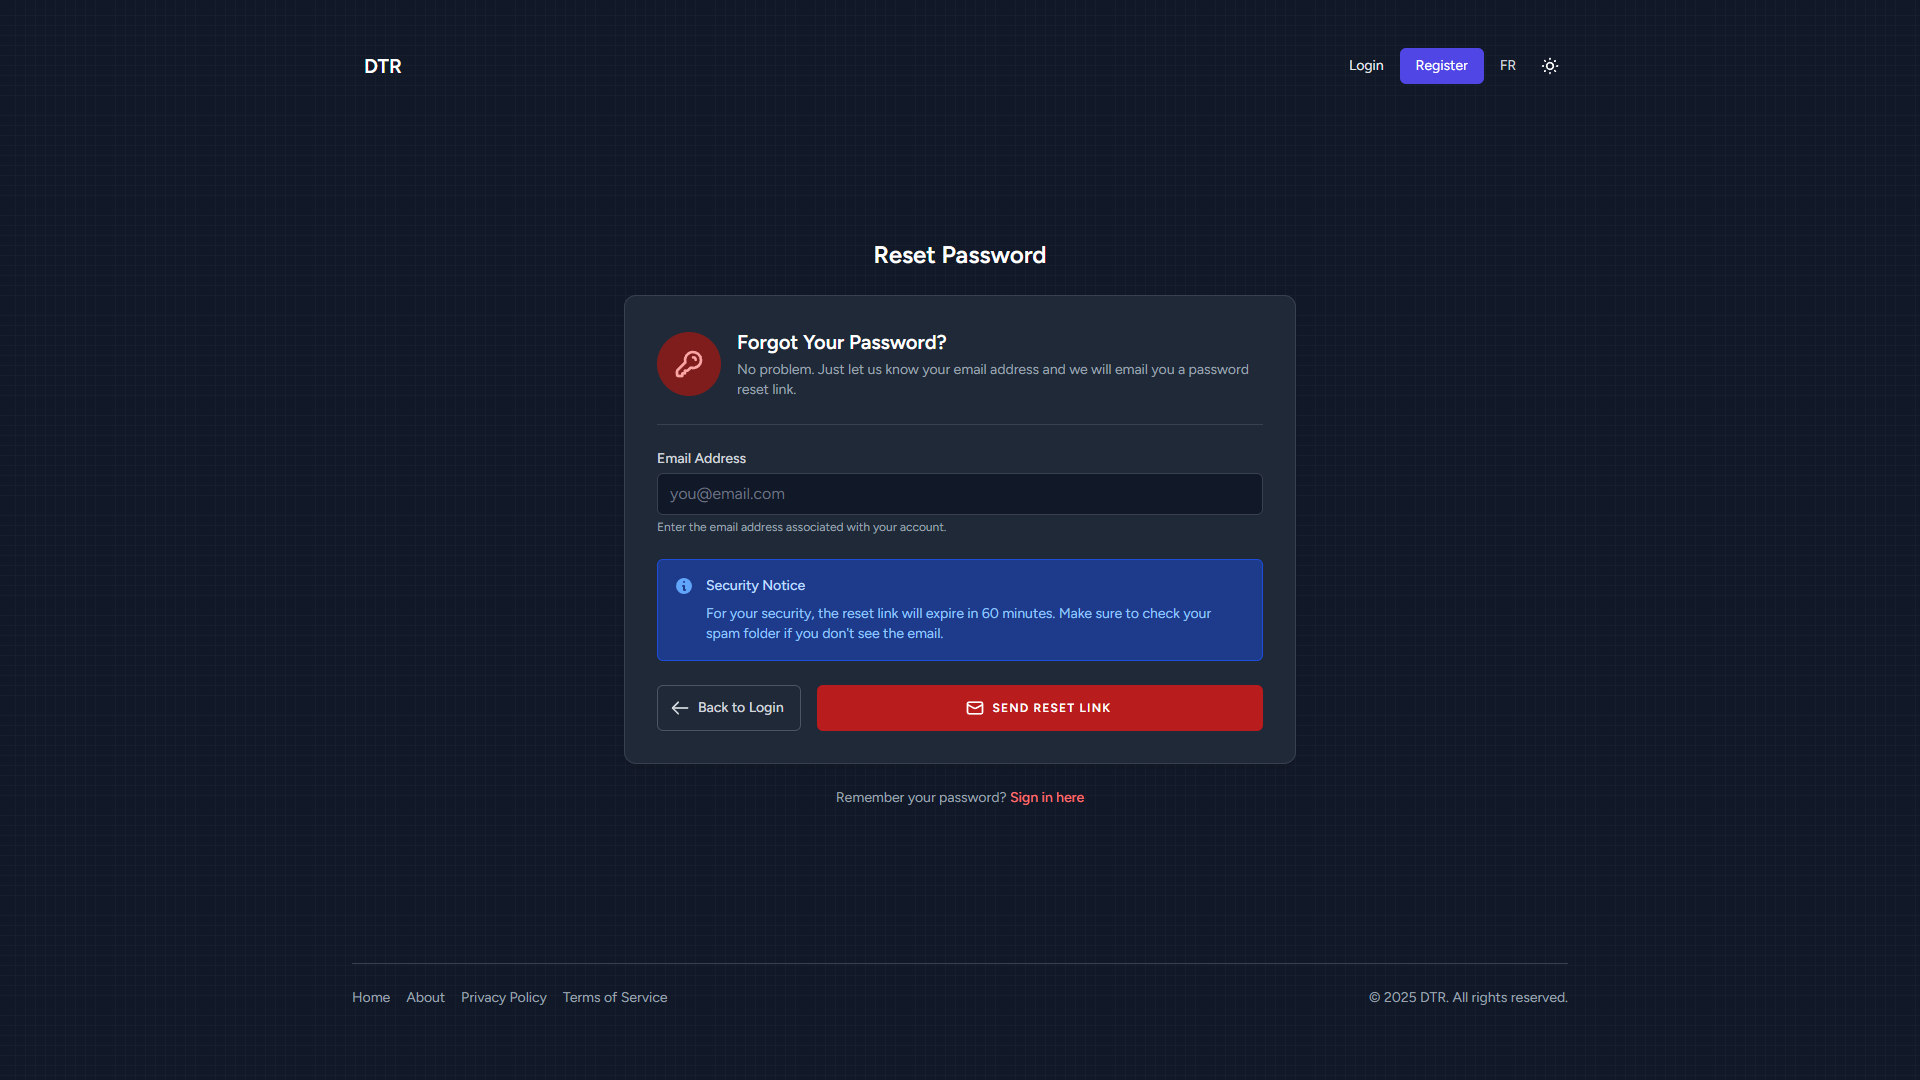
\includegraphics[width=0.85\textwidth]{assets/chapter4/screenshots/iotreap-quiz-engine.png}
\caption{Quiz Engine Attempt and Grading Interface}
\label{fig:quiz-engine}
\end{figure}

\subsection{Notifications Module}

The notifications module provides real-time and persistent notification delivery to keep users informed about platform events relevant to their role and activity. Notifications cover a wide range of events including enrollment confirmations, session expiration warnings, payment receipts, certificate generation, content approval decisions, and forum replies.

The implementation uses a database-backed notification store with read-state tracking, allowing users to view both unread and historical notifications. The frontend renders notifications through a dedicated panel accessible from the application header, with badge indicators for unread counts. Notifications are also dispatched via email for critical events, ensuring that important information reaches users even when they are not actively using the platform.

Real-time event delivery is implemented through Laravel Reverb, a first-party WebSocket server that broadcasts platform events to connected browsers. The CustomDatabaseChannel handles notification persistence, while the broadcast authorization channels defined in the routing configuration ensure that users only receive events relevant to their sessions and roles. The platform defines nine notification types covering the principal event categories: payout approval and rejection notifications for teachers, refund approval and rejection notifications for learners, session activation failure alerts for engineers, teacher account pending approval notifications for administrators, training path approval and rejection notifications for content authors, and USB device availability notifications for engineers awaiting hardware access.

\begin{figure}[H]
\centering
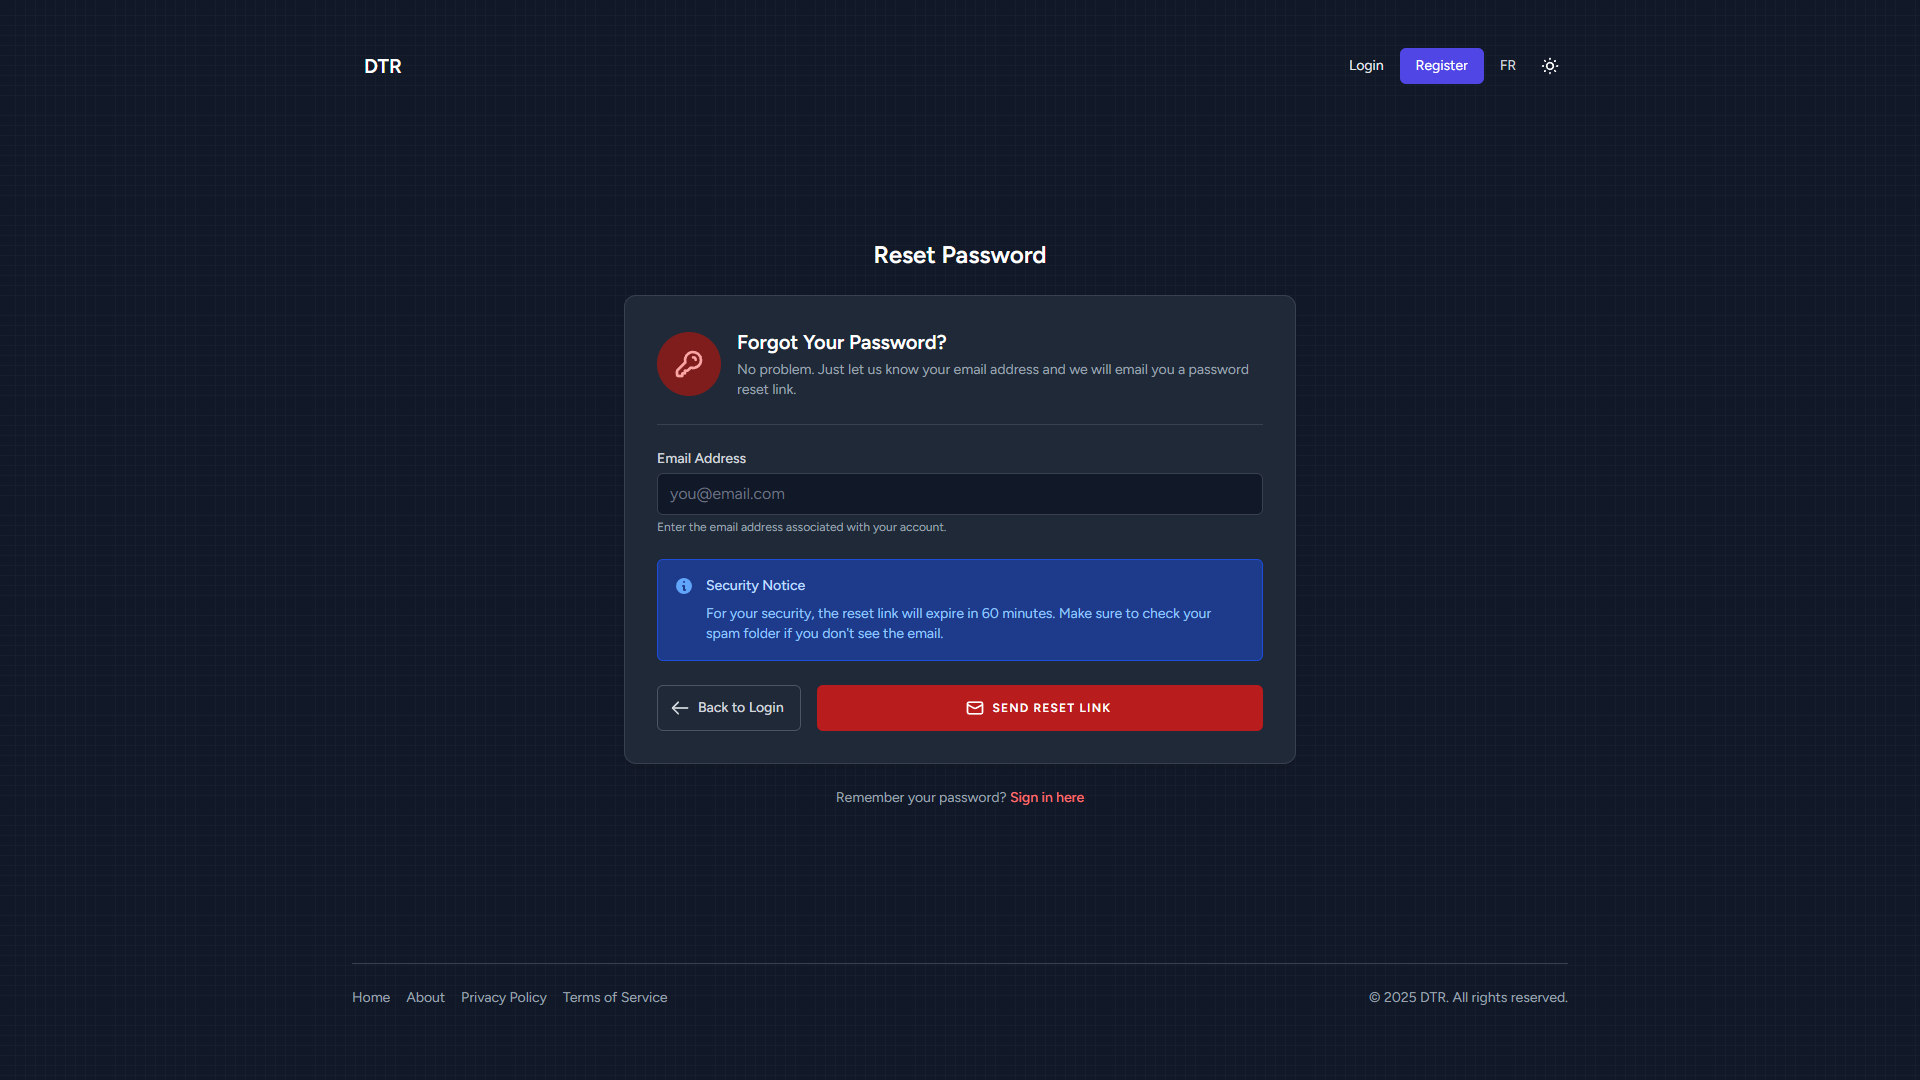
\includegraphics[width=0.85\textwidth]{assets/chapter4/screenshots/iotreap-notifications.png}
\caption{Notifications Panel}
\label{fig:notifications}
\end{figure}

\subsection{Certificate Generation and Verification}

The certificate module generates formal proof of training path completion for learners who have satisfied all unit requirements. Certificates are produced as downloadable documents containing the learner's name, the training path title, the completion date, and a unique verification code.

A key implementation feature is the public verification endpoint, which allows third parties to confirm the authenticity of a certificate by entering its verification code on a public page. This mechanism adds formal credibility to the training delivered through IoT-REAP and supports professional recognition of the skills acquired.

\begin{figure}[H]
\centering
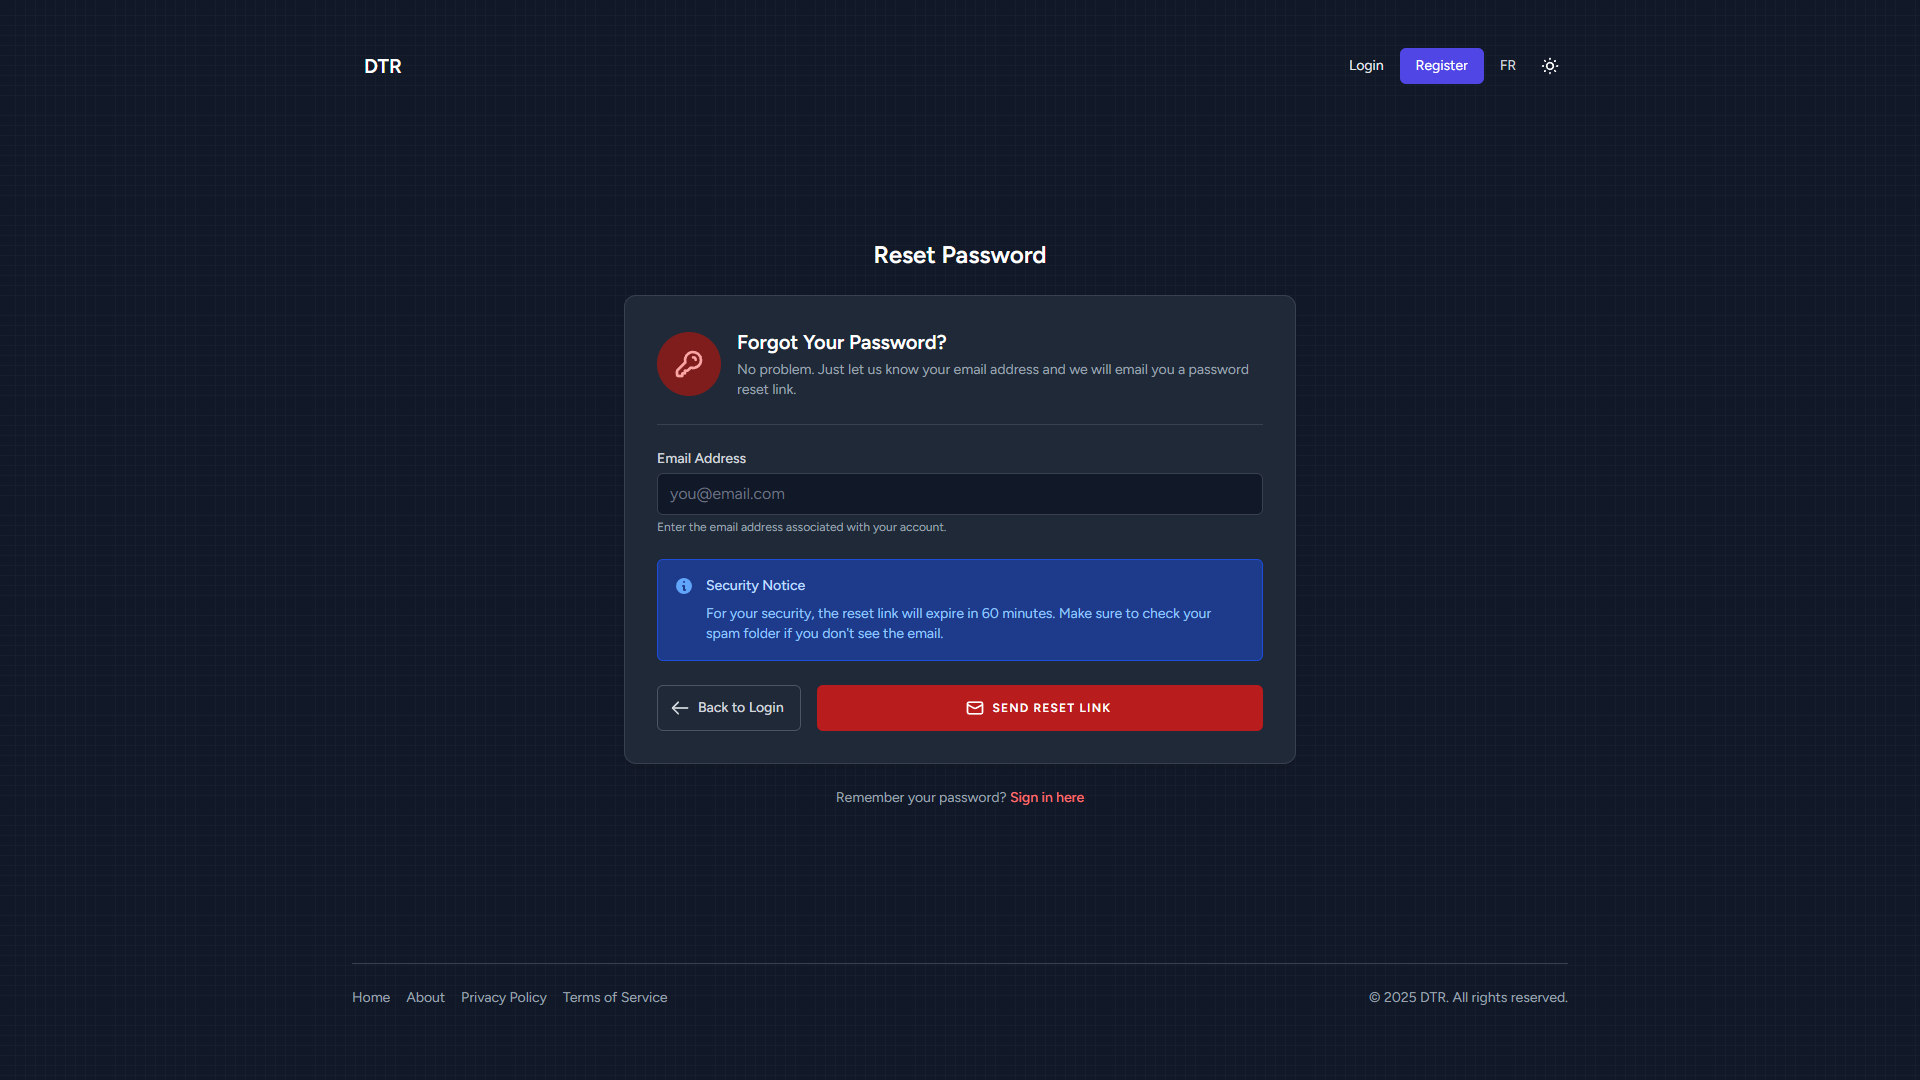
\includegraphics[width=0.85\textwidth]{assets/chapter4/screenshots/iotreap-certificate.png}
\caption{Certificate Generation and Verification Interface}
\label{fig:certificate}
\end{figure}

\subsection{Payment and Checkout Interface}

The payment module integrates Stripe to handle secure financial transactions for training path enrollment. The checkout flow creates a Stripe Checkout Session, redirects the user to the Stripe-hosted payment page, and processes the webhook callback to confirm payment completion and trigger automatic enrollment.

The implementation includes webhook signature verification to prevent spoofed payment confirmations, idempotent handling of duplicate webhook events, and administrative interfaces for refund processing and payout management. Instructors can track their earnings and request payouts through the teaching dashboard, while administrators oversee the full financial lifecycle including refund approvals and payout execution.

The Stripe webhook handler illustrates how the platform processes payment completion events. When a checkout session completed event is received, the handler looks up the corresponding payment record by the Stripe session identifier. If no matching payment is found, a warning is logged and processing stops. If the payment has already been marked as completed---which can occur when Stripe sends duplicate webhook events---the handler logs an informational message and exits idempotently. Otherwise, the payment is marked as completed with the Stripe payment intent identifier, and the user is automatically enrolled in the corresponding training path. Each step is logged with contextual details to support financial auditing and operational debugging.

\begin{figure}[H]
\centering
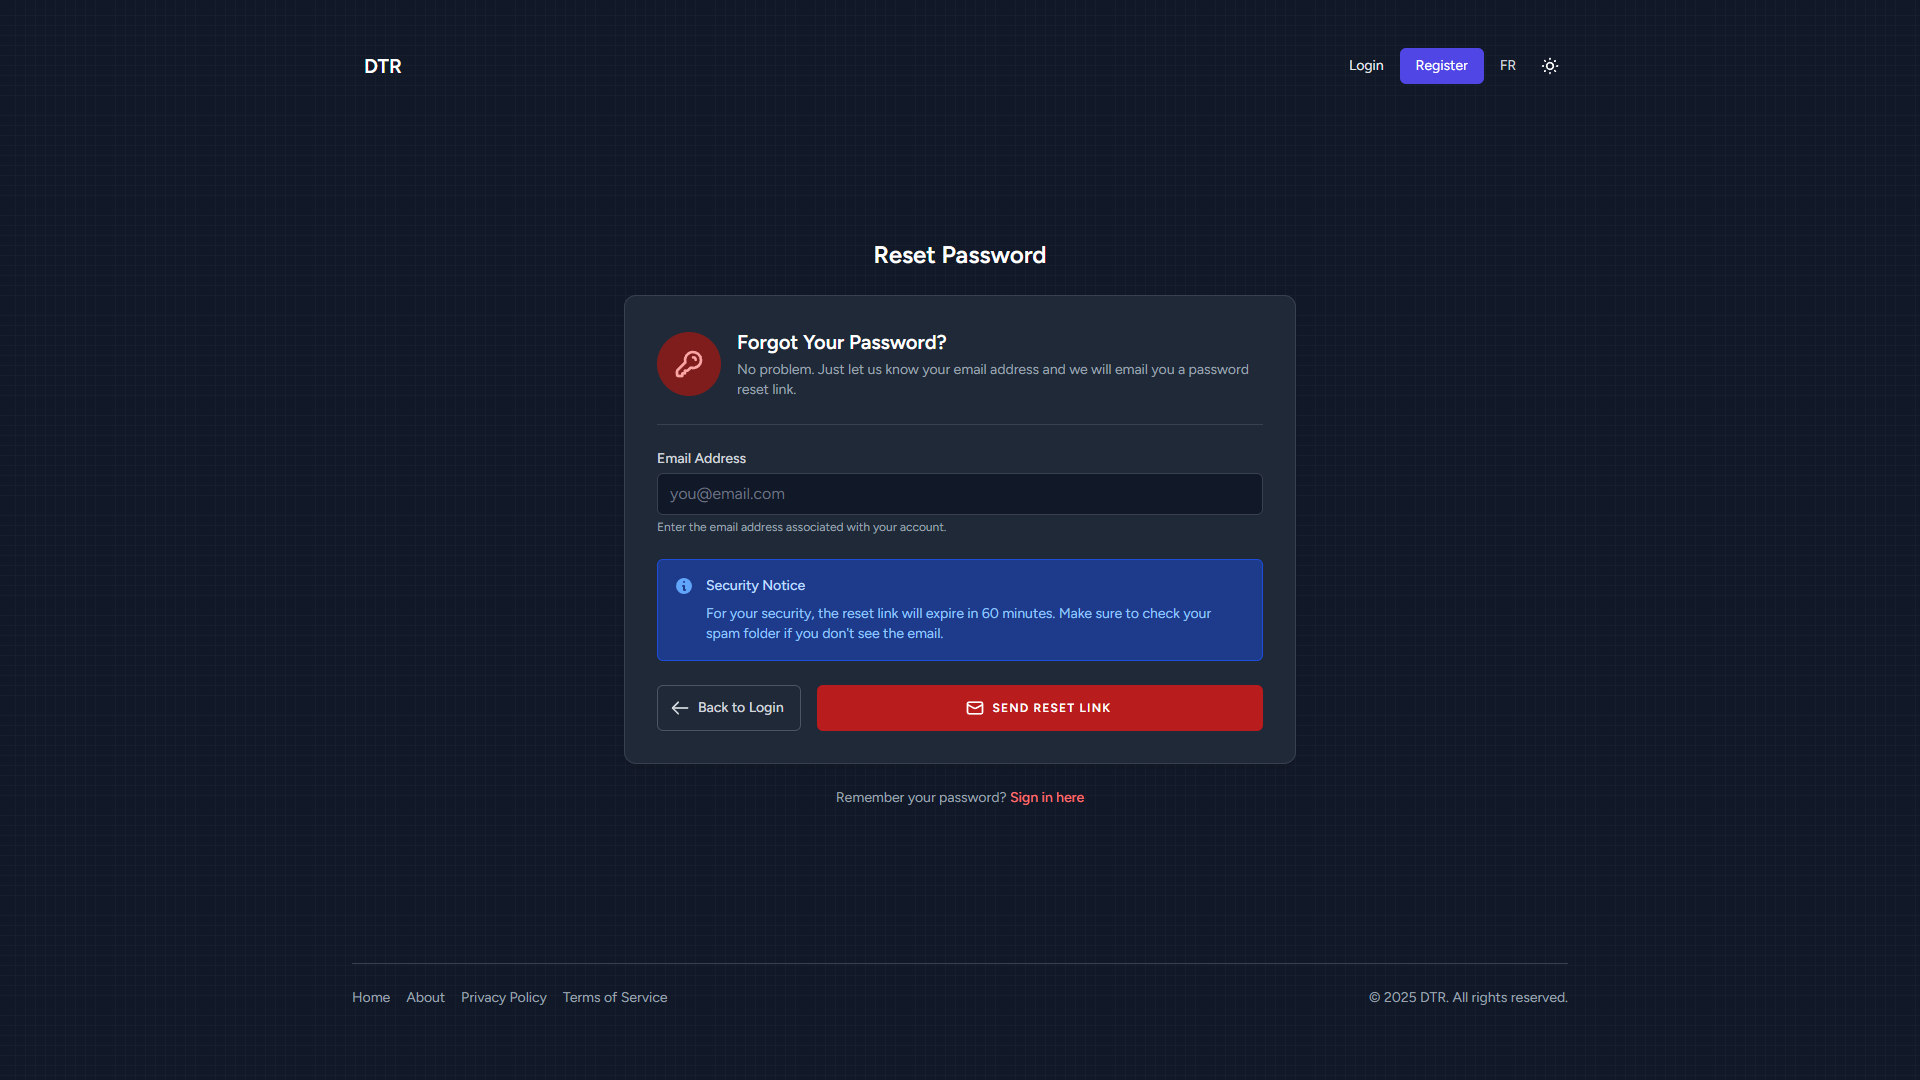
\includegraphics[width=0.85\textwidth]{assets/chapter4/screenshots/iotreap-payment-checkout.png}
\caption{Payment and Checkout Flow}
\label{fig:payment-checkout}
\end{figure}

\subsection{Reservation Management Interface}

The reservation module enables users to book shared physical resources such as cameras and hardware devices for specific time slots. This is critical in environments where training equipment is limited and must be shared fairly among multiple users.

The implementation includes availability checking, conflict prevention, reservation creation and cancellation, and administrative oversight for managing reservation policies. Users receive notifications about upcoming reservations and expiration reminders, while administrators can review reservation utilization patterns and adjust resource allocation accordingly.

\begin{figure}[H]
\centering
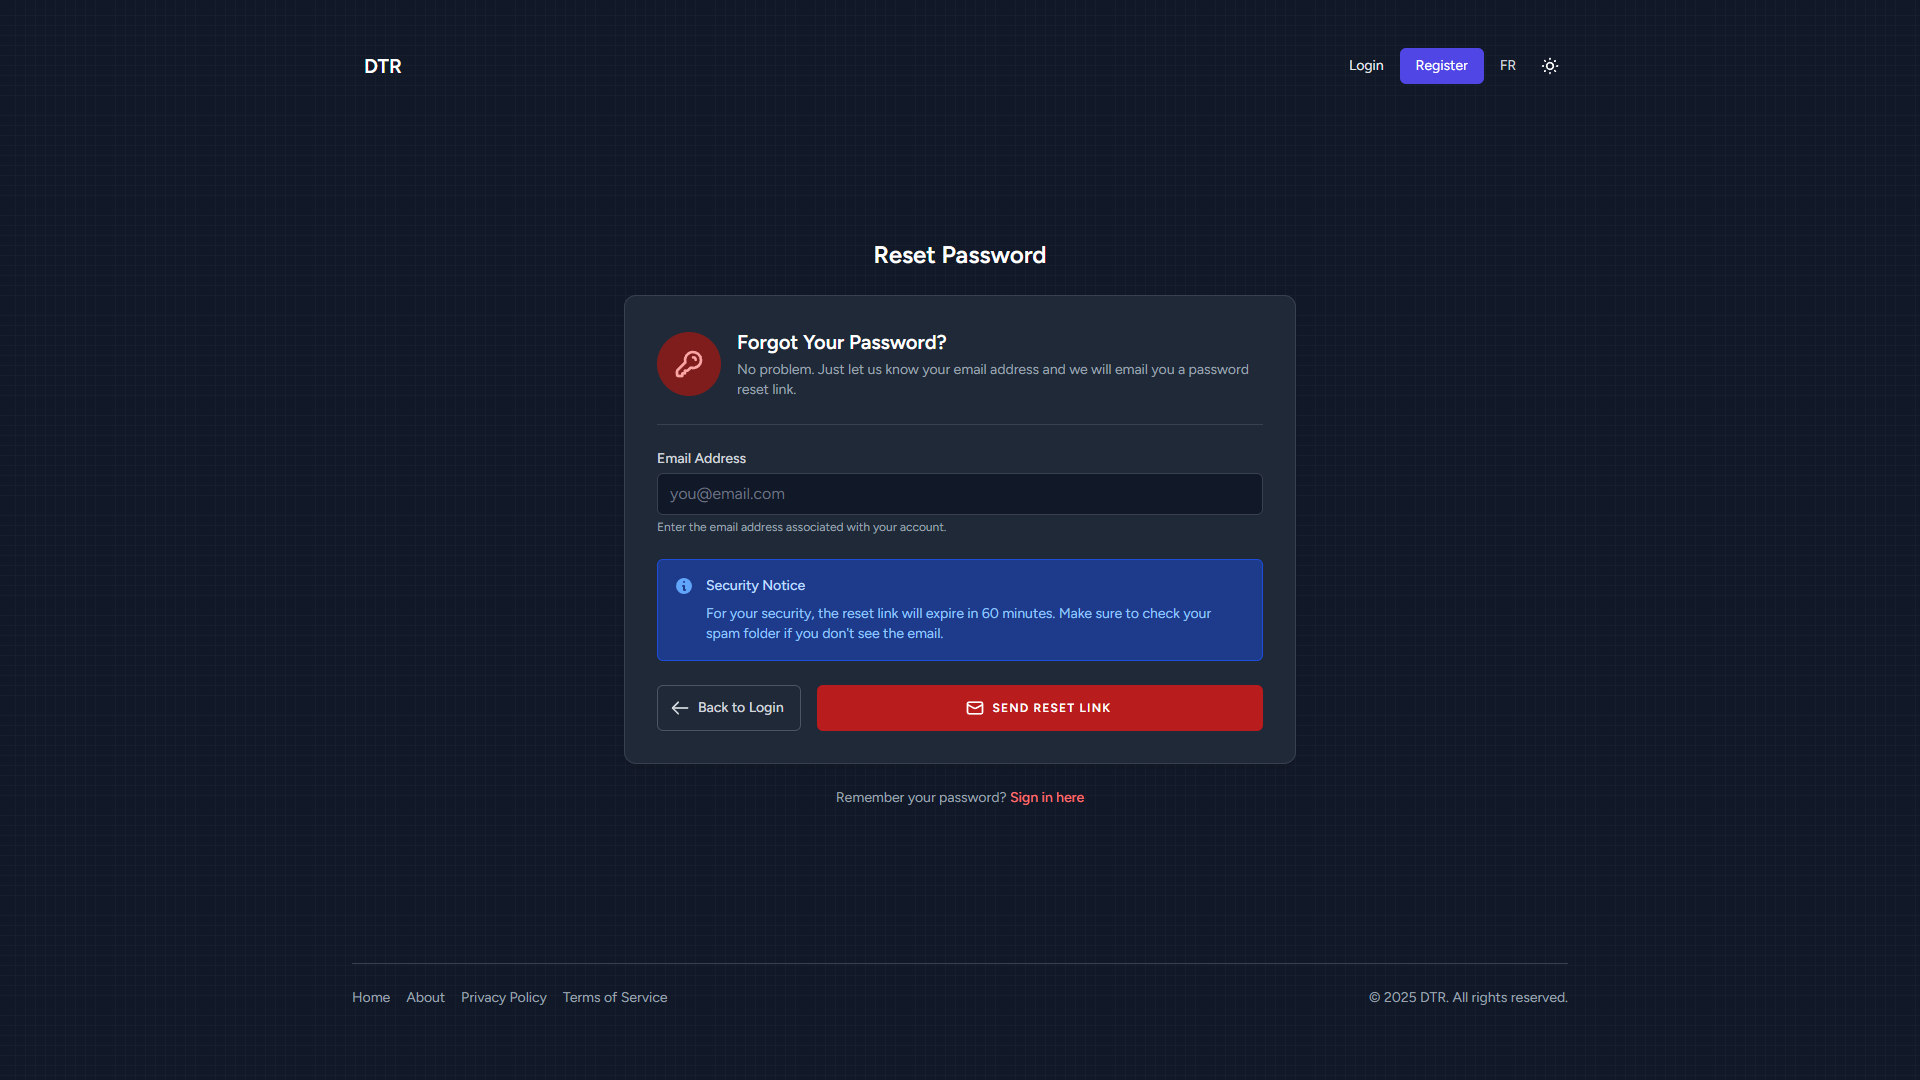
\includegraphics[width=0.85\textwidth]{assets/chapter4/screenshots/iotreap-reservations.png}
\caption{Reservation Management Interface}
\label{fig:reservations}
\end{figure}

\section*{Conclusion}
\addcontentsline{toc}{section}{Conclusion}

This chapter presented the technical environment and the main realized modules of IoT-REAP, including authentication, remote sessions, learning interfaces, teaching workflows, administration, reservations, video streaming, quizzes, certificates, payments, and hardware-related features.

\cleardoublepage
